% === CONTEXTO === %

\vspace{1em}
\subsection{Contexto}

La red del \textit{Club de Karate} fue parte de una investigación antropológica \cite{Zachary}, realizada por Wayne W. Zachary, que estudió las relaciones `políticas' entre los miembros de un club universitario. La misma se realizó durante el desarrollo de un conflicto que terminó por dividir al grupo. 

La red buscó modelar el flujo de información entre sus integrantes por medio de la tripla $(\mathbf{V},\ \mathbf{E},\ \mathbf{C})$, donde $\mathbf{V}$ denota el conjunto de individuos, $\mathbf{E}$ refiere a un grafo no direccionado cuyos ejes representan los vínculos entre los miembros del club, y $\mathbf{C}$ define la fuerza de estas relaciones ---lo que se podría pensar como ponderaciones sobre los ejes de $\mathbf{E}$---. 

\vspace{1em}
La investigación tuvo como enfoque central demostrar la capacidad del modelo para predecir la división del grupo por medio del algoritmo de \textit{labeling} de `flujo máximo - corte mínimo' de Ford y Fulkerson \cite{Ford}.

\vspace{1em}
\begin{figure}[!htbp]
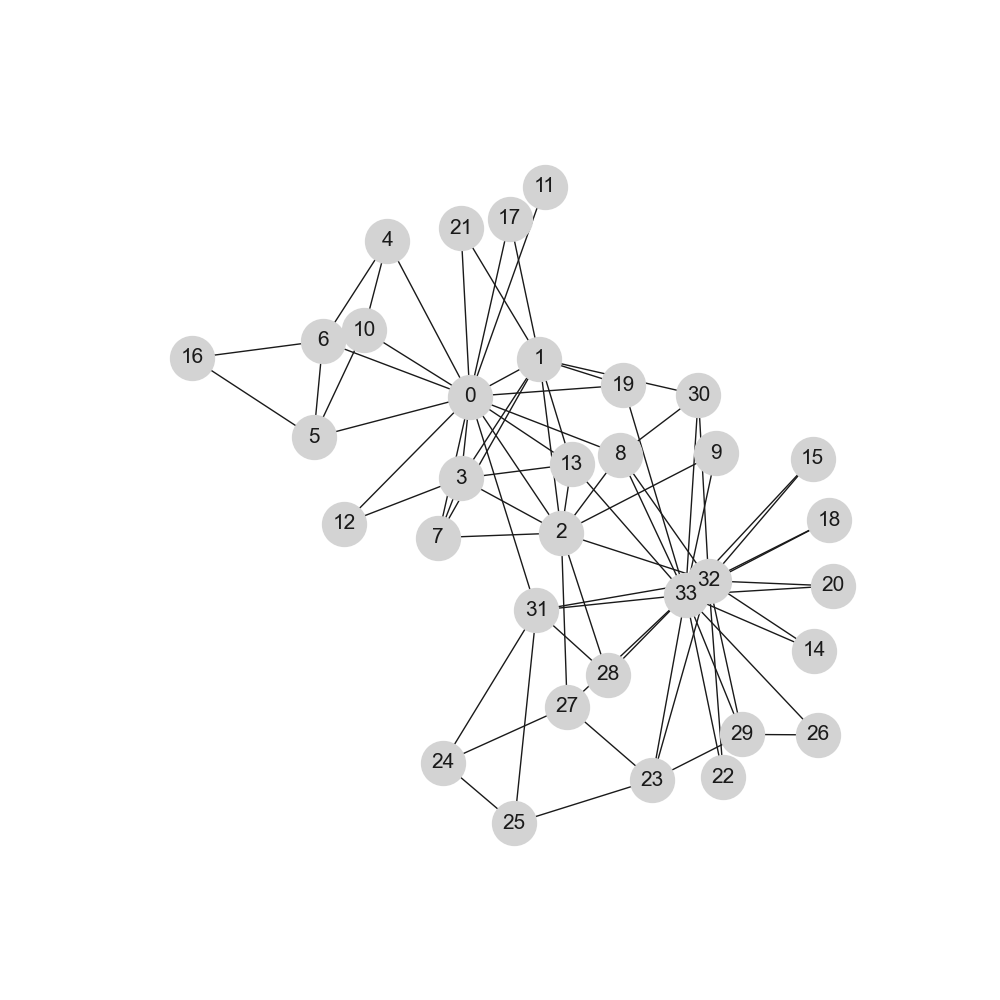
\includegraphics[scale=0.55, trim=100 80 100 100, clip]{/files/src/.media/grafo_conectividad.png}
\caption{La red del \textit{Club de Karate}. Cada nodo representa un individuo, cada eje la existencia de un vínculo por fuera del club.}
\end{figure}


\vspace{1em}
En este análisis\footnote{El script asociado se puede encontrar en \textit{./experimentos/club\_de\_karate.py}, los archivos con los resultados en \textit{./experimentos/resultados/club-karate/}.} utilizaremos sólo la representación matricial de $\mathbf{E}$ para evaluar la importancia de los distintos miembros en la red, y la matriz laplaciana asociada para evaluar el uso de autovectores como predictores de la división del grupo. 




% === CENTRALIDAD DE AV === %
\newpage
\vspace{2em}
\subsection{Centralidad de Autovector} La centralidad de autovector es una medida que se utiliza en el análisis de redes para medir la `importancia' de los nodos que componen una red, relativa a la importancia de sus conexiones. Dada una matriz de conectividad \textbf{W}, se define:

\vspace{1em}
\begin{equation} \label{conectividad}
    \lambda x = \mathbf{W} x
\end{equation}

\vspace{1em}
\noindent donde $\lambda$ es el autovalor en módulo máximo de \textbf{W}.

\vspace{1em}
Intuitivamente, se puede pensar que la importancia de cada nodo es proporcional a la suma de las importancias de sus vecinos. Se puede demostrar  \cite{Newman} que, dado las características de esta matriz, el autovector asociado siempre será positivo en coordenadas.

\vspace{1em}
En tanto la red de \textit{Club de Karate}, podemos ver que la aplicación del metodo de la potencia sobre la matriz de conectividad asociada al grafo $\mathbf{E}$ resulta en el siguiente autovector asociado al autovalor en módulo máximo:

\vspace{1em}
\begin{figure}[!htbp]
\begin{equation*} 
    \begin{bmatrix}
        0   &0.355491 \\
        1   &0.265960 \\
        2   &0.317193 \\
        3   &0.211180 \\
        4   &0.075969 \\
        5   &0.079483 \\
        6   &0.079483 \\
        7   &0.170960 \\
        8   &0.227404 \\
        9   &0.102674 \\
        10  &0.075969 \\
        11  &0.052856 \\
        12  &0.084255 \\
        13  &0.226473 \\
        14  &0.101403 \\
        15  &0.101403 \\
        16  &0.023636 \\
    \end{bmatrix}
    \begin{bmatrix}
        17  &0.092400 \\
        18  &0.101403 \\
        19  &0.147913 \\
        20  &0.101403 \\
        21  &0.092400 \\
        22  &0.101403 \\
        23  &0.150119 \\
        24  &0.057052 \\
        25  &0.059206 \\
        26  &0.075579 \\
        27  &0.133477 \\
        28  &0.131078 \\
        29  &0.134961 \\
        30  &0.174758 \\
        31  &0.191034 \\
        32  &0.308644 \\
        33  &0.373363 \\
    \end{bmatrix}
\end{equation*}
\caption{Centralidad de autovector para la red del \textit{Club de Karate}. La columna izquierda denota el nodo, la derecha su `importancia'.} \label{centralidad_karate}
\end{figure}

\vspace{1em}
Vemos que el nodo `0' y el nodo `33' son los más centrales. Esto no es casualidad, la red del \textit{Club de Karate} está armada para tener a las dos figuras principales del conflicto en cada extremo ---el instructor de karate y el presidente del club, respectivamente--- para satisfacer la especificación del algoritmo de labeling que utiliza.




% === AV DE LA MATRIZ LAPLACIANA === %

\vspace{2em}
\subsection{Autovectores de la matriz laplaciana} La matriz laplaciana $\mathbf{L} = \mathbf{D} - \mathbf{W}$ ---donde \textbf{D} es una matriz diagonal con elementos $d_{ii} = \sum_j w_{ij}$ y \textbf{W} es una matriz de conectividad--- sirve para medir distintas propiedades en una red. 

En particular, el mínimo autovalor en módulo no nulo ---llamado de conectividad algebráica, o valor de Fiedler--- permite establecer un criterio sobre el que particionar la red en dos. El autovector asociado a este autovalor designará la pertenencia de un nodo a una u otra partición acorde a su signo. 

\vspace{1em}
Procedemos a analizar qué autovector de la matriz laplaciana asociada a $\mathbf{E}$ permite predecir mejor la división que ocurrió en el \textit{Club de Karate}. Para ello, calculamos los autovectores de la matriz laplaciana con el método de la potencia con deflación y medimos el valor absoluto de la correlación entre cada autovector y un vector que indica la división verdadera que ocurrió en el grupo.

\vspace{1em}
\begin{figure}[!htbp]
\begin{equation*} 
    \begin{bmatrix}
        18.136696 & 0.266429 \\
        17.055171 & 0.066721 \\
        13.306122 & 0.457220 \\
        10.921068 & 0.339844 \\
        9.777241  & 0.496086 \\
        6.996197  & 0.060813 \\
        6.515545  & 0.461652 \\
        6.331592  & 0.082665 \\
        5.618034  & 0.0 \\
        5.378595  & 1.427676 \\
        4.580793  & 0.465710 \\
        4.480008  & 0.262230 \\
        4.275877  & 0.062841 \\
        3.472187  & 0.001872 \\
        3.381966  & 0.0 \\
        3.376154  & 0.379940 \\
        3.242067  & 0.505417 
    \end{bmatrix}
    \begin{bmatrix}
        3.013963 & 0.055720 \\
        2.749157 & 0.940899 \\
        2.487092 & 0.684434 \\
        2.0 & 0.0 \\
        2.0 & 0.0 \\
        2.0 & 0.0 \\
        2.0 & 0.0 \\
        2.0 & 0.0 \\
        1.955050 & 0.065144 \\
        1.826055 & 0.401069 \\
        1.761899 & 0.158209 \\
        1.599283 & 0.325133 \\
        1.259404 & 0.002377 \\
        1.125011 & 1.943500 \\
        0.909248 & 1.550553 \\
        0.468525 & 4.750632 \\
        0.0 & nan\footnotemark
    \end{bmatrix}
\end{equation*}
\caption{Correlación entre los autovectores asociados a los autovalores de la red del \textit{Club de Karate} y un vector que indica la división verdadera que ocurrió en el grupo. La columna izquierda denota el autovalor, la derecha la correlación.} \label{conectividad_karate}
\end{figure}
\footnotetext{El método de la potencia no está definido si el autovalor máximo en módulo es nulo. Este resultado da cuenta de ello. Como nos interesan solo los autovalores diferentes a `0', optamos por descartarlo.}

\vspace{1em}
Vemos que el valor de conectividad algebráica ---el autovalor mínimo en módulo no nulo--- tiene asociado el mejor autovector para realizar el corte. En la figura (\ref{prediccion_karate}.) se puede observar que sólo dos nodos obtuvieron una clasificación incorrecta: el `2' y el `8', lo que presenta un desempeño casi igual al logrado en la investigación original\footnote{En este sentido, solo el nodo `2' recibió una clasificación incorrecta. Sobre el `8', Zachary considera \cite{Zachary} que hubo un interés `egoísta', por parte del individuo asociado a ese nodo, que lo hizo actuar de manera distinta a su `afiliación' política (es decir, sus relaciones).}.

\newpage
\vspace{2em}
\begin{figure}[!htbp]
\begin{equation*}
    \begin{bmatrix}
        0   &-0.112137 & 0 & 0 \\ 
        1   &-0.041288 & 0 & 0 \\
        2   &0.023219 & 1 & 0 \\
        3   &-0.055500 & 0 & 0 \\
        4   &-0.284605 & 0 & 0 \\
        5   &-0.323727 & 0 & 0 \\
        6   &-0.323727 & 0 & 0 \\
        7   &-0.052586 & 0 & 0 \\
        8   &0.051601 & 1 & 0 \\
        9   &0.092801 & 1 & 1 \\
        10  &-0.284605 & 0 & 0 \\
        11  &-0.210993 & 0 & 0 \\
        12  &-0.109461 & 0 & 0 \\
        13  &-0.014742 & 0 & 0 \\
        14  &0.162751 & 1 & 1 \\
        15  &0.162751 & 1 & 1 \\
        16  &-0.422765 & 0 & 0 \\
    \end{bmatrix}
    \begin{bmatrix}
        17  &-0.100181 & 0 & 0 \\
        18  &0.162751 & 1 & 1 \\
        19  &-0.013637 & 0 & 0 \\
        20  &0.162751 & 1 & 1 \\
        21  &-0.100181 & 0 & 0 \\
        22  &0.162751 & 1 & 1 \\
        23  &0.155695 & 1 & 1 \\
        24  &0.153026 & 1 & 1 \\
        25  &0.160963 & 1 & 1 \\
        26  &0.187110 & 1 & 1 \\
        27  &0.127664 & 1 & 1 \\
        28  &0.095152 & 1 & 1 \\
        29  &0.167650 & 1 & 1 \\
        30  &0.073500 & 1 & 1 \\
        31  &0.098753 & 1 & 1 \\
        32  &0.130345 & 1 & 1 \\
        33  &0.118903 & 1 & 1 \\
    \end{bmatrix}
\end{equation*}
\caption{Autovector de Conectividad algebráica, la primer columna representa los nodos de la red, la segunda el autovector, la tercera la clasificación de cada nodo acorde a su signo y la cuarta la división verdadera que ocurrió.} \label{prediccion_karate}
\end{figure}

\vspace{1em}
\begin{figure}[!htbp]
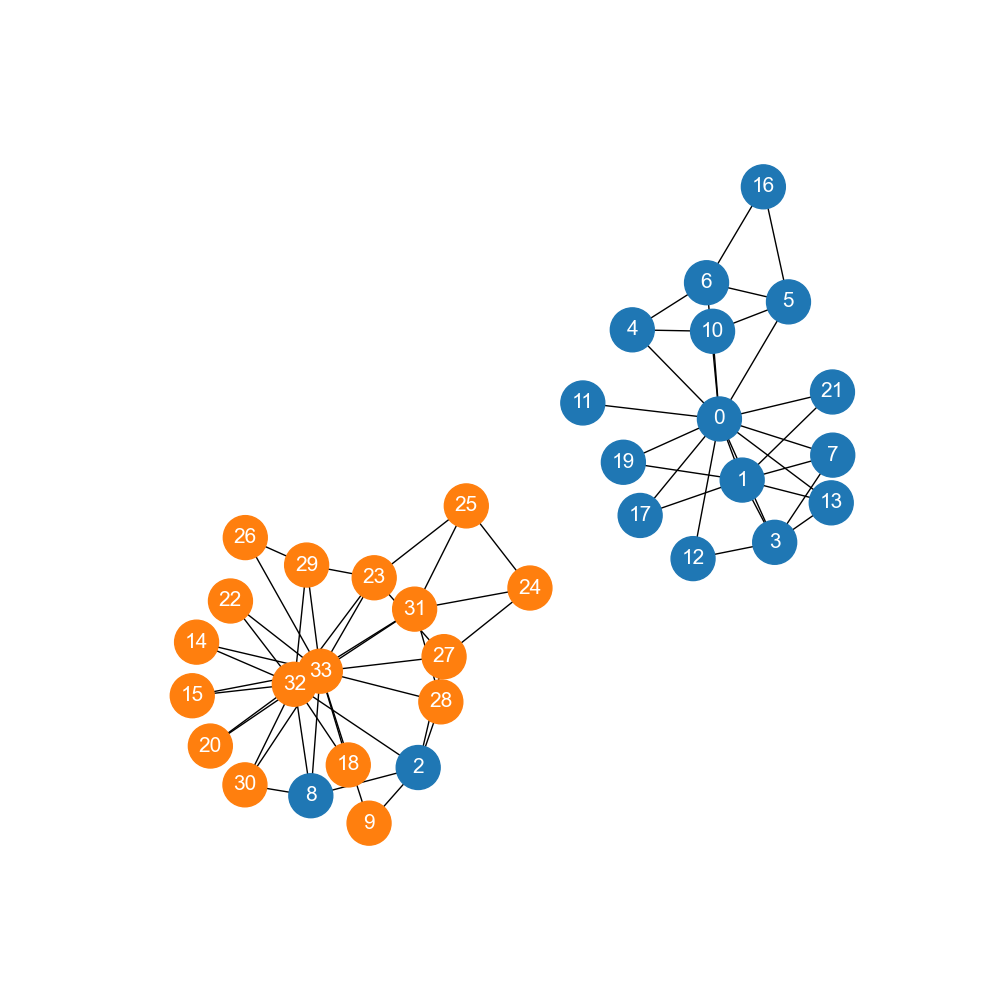
\includegraphics[scale=0.5, trim=100 90 100 100, clip]{/files/src/.media/grafo_corte_32_0.47.png}
\caption{La división estimada de la red del \textit{Club de Karate}. Los colores representan la división verdadera de la red. Azul: `0', Naranja: `1'.}
\end{figure}

\vspace{1em}
Procedemos a detallar ---a modo de comparación visual--- los cortes realizados por los demás autovectores. Notamos que el proceso de corte sólo elimina los ejes existentes entre pares cuya clasificación difiere. Por ello, la cantidad de componentes conexos que puede generar un corte no es necesariamente dos.  

\begin{figure}[!htbp]
    \centering
    \subfloat[av $\approx$ 0.91]{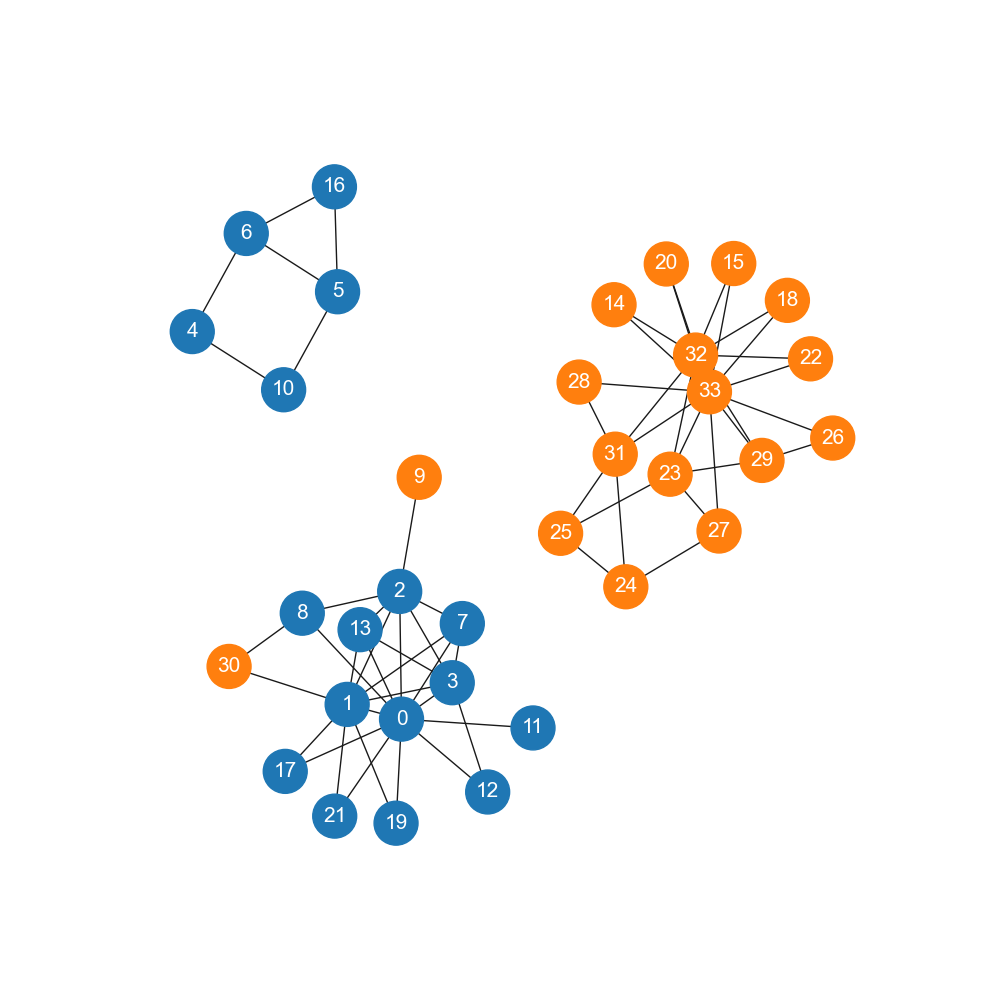
\includegraphics[width=.25\textwidth]{/files/src/.media/grafo_corte_31_0.91.png}}\hfill
    \subfloat[av $\approx$ 1.13]{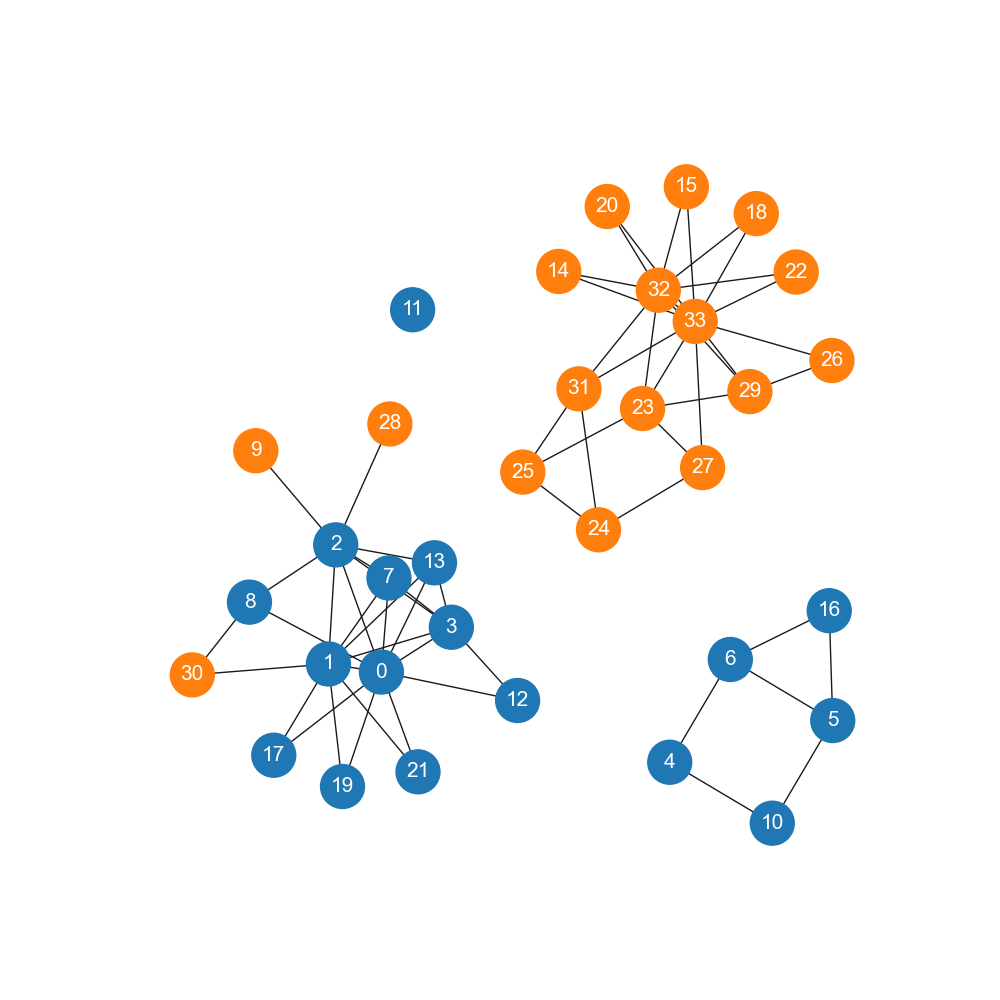
\includegraphics[width=.25\textwidth]{/files/src/.media/grafo_corte_30_1.13.png}}\hfill
    \subfloat[av $\approx$ 1.26]{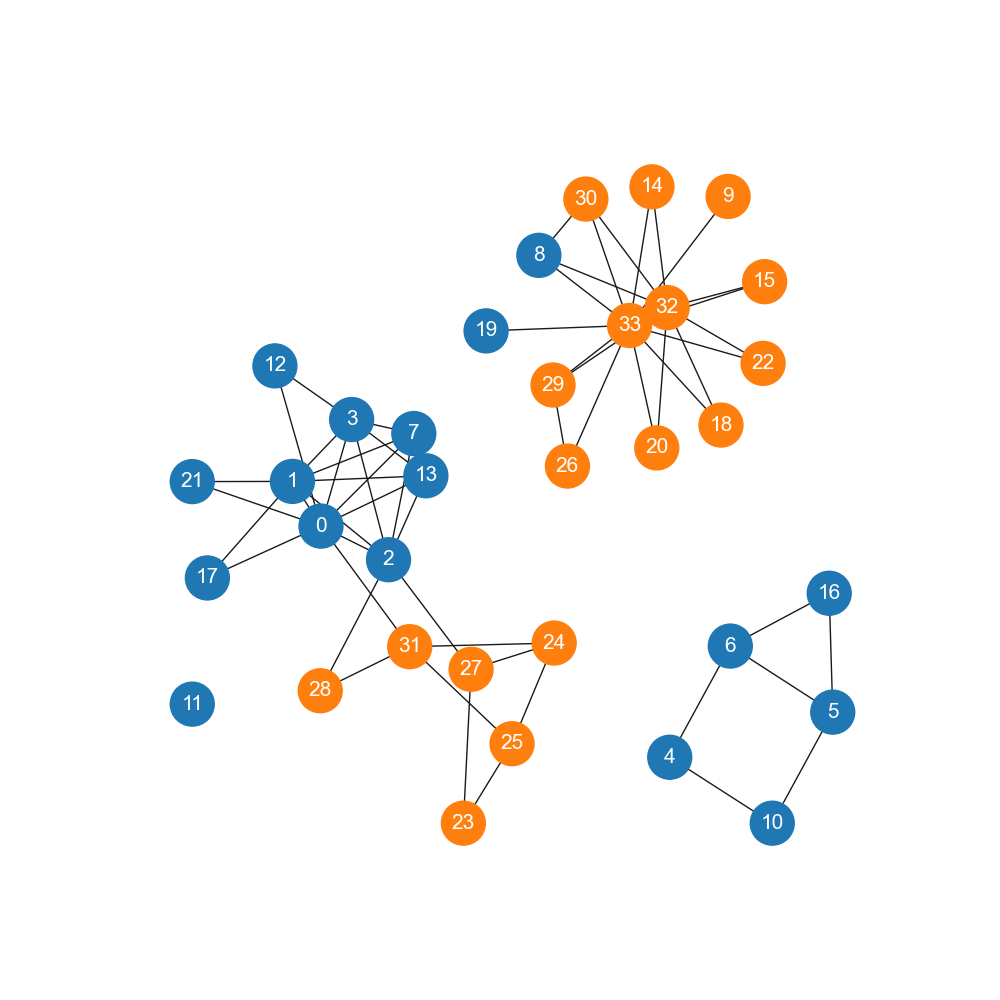
\includegraphics[width=.25\textwidth]{/files/src/.media/grafo_corte_29_1.26.png}}\hfill
    \subfloat[av $\approx$ 1.60]{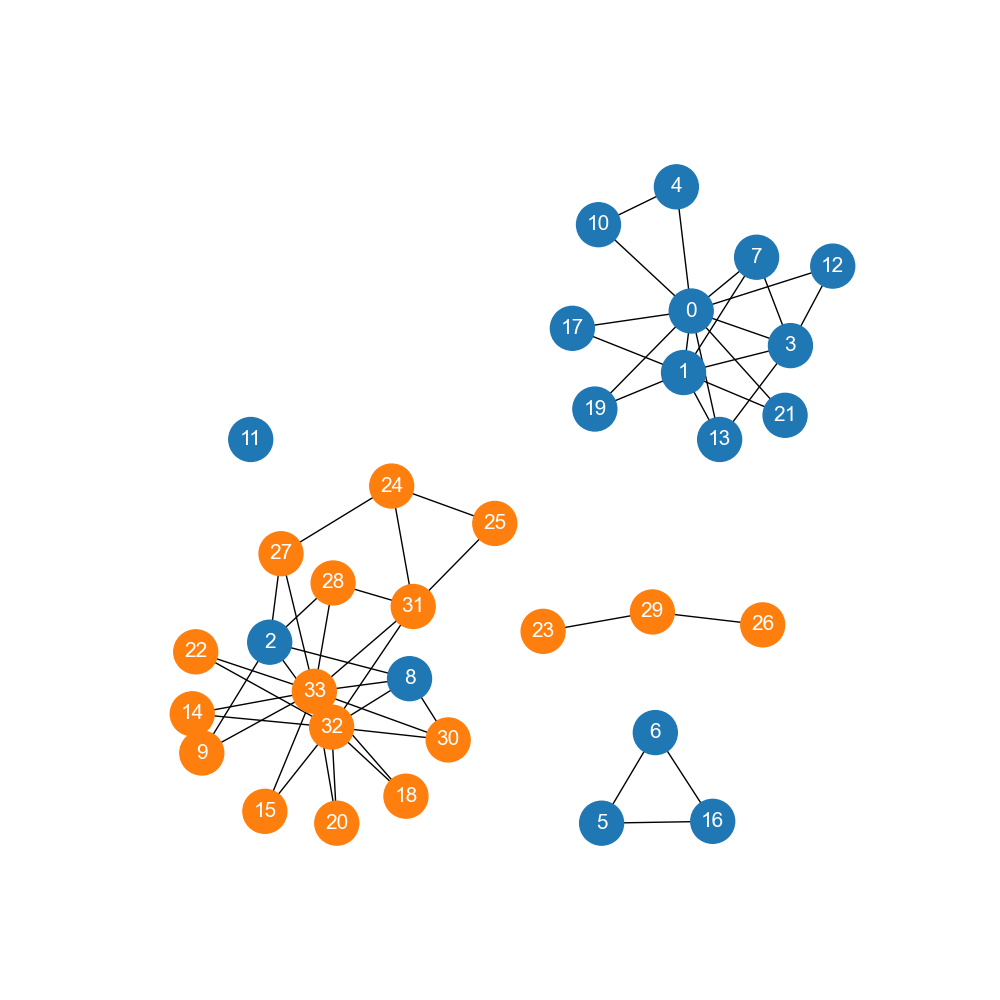
\includegraphics[width=.25\textwidth]{/files/src/.media/grafo_corte_28_1.6.png}}\hfill
    \\[\smallskipamount]
    \subfloat[av $\approx$ 1.76]{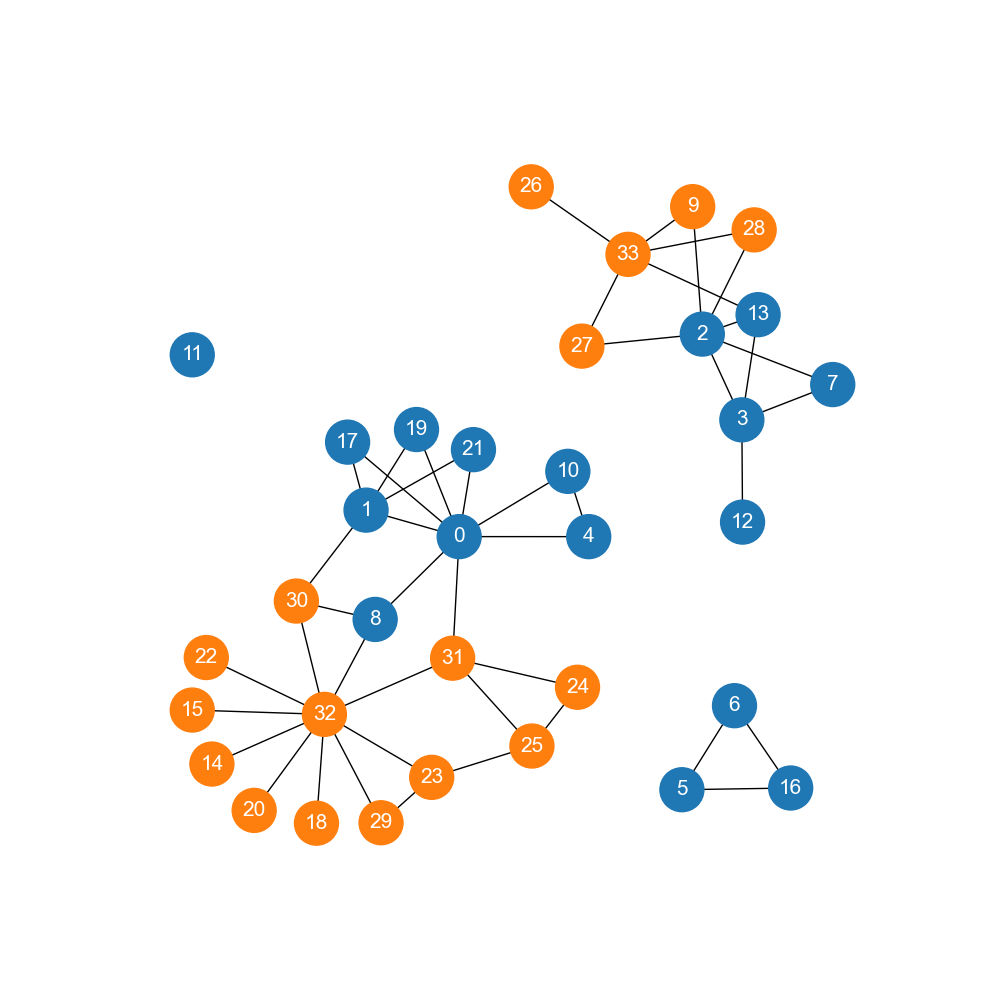
\includegraphics[width=.25\textwidth]{/files/src/.media/grafo_corte_27_1.76.png}}\hfill
    \subfloat[av $\approx$ 1.83]{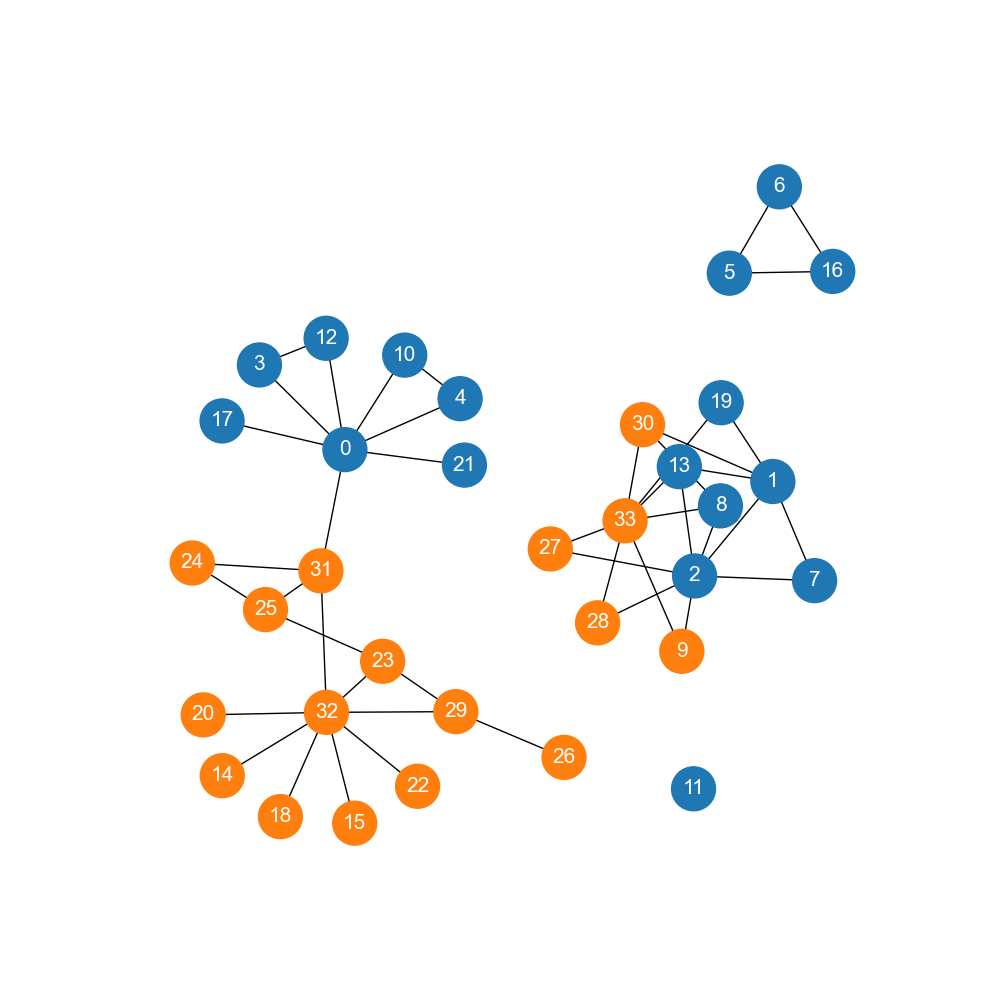
\includegraphics[width=.25\textwidth]{/files/src/.media/grafo_corte_26_1.83.png}}\hfill
    \subfloat[av $\approx$ 1.96]{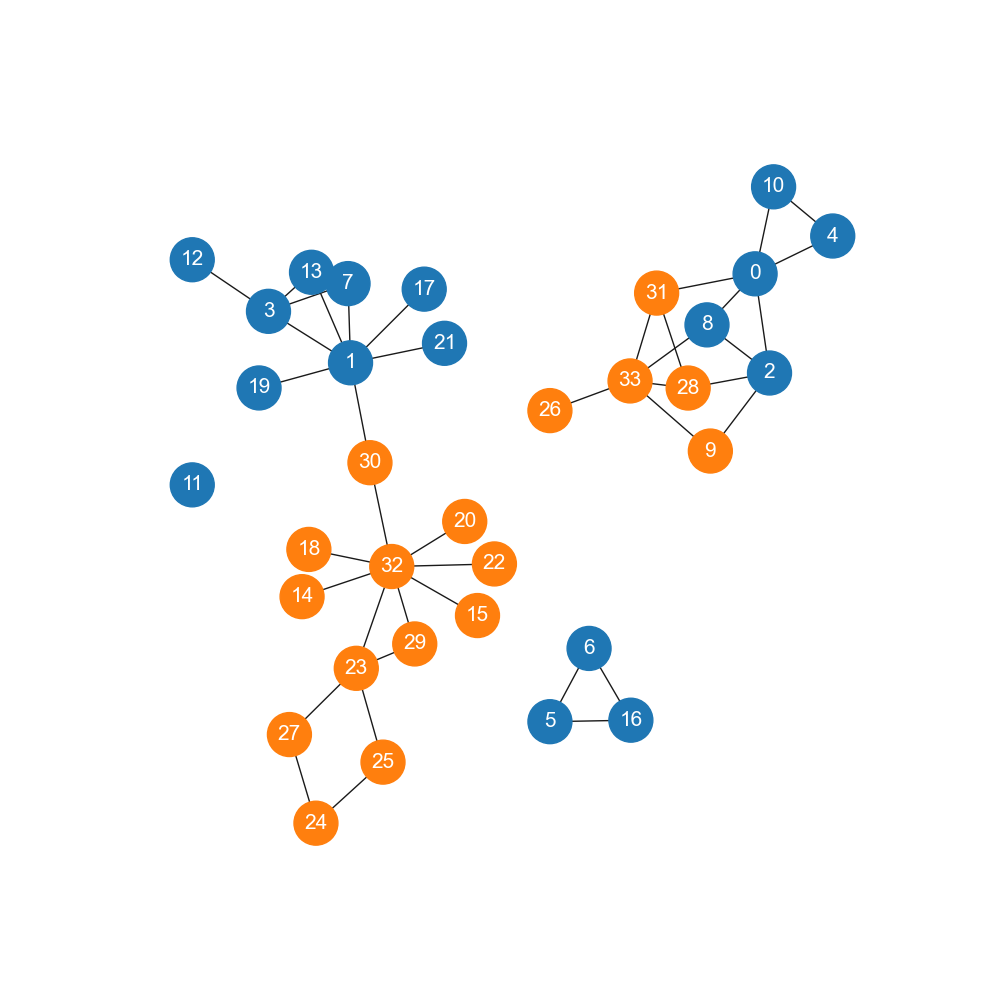
\includegraphics[width=.25\textwidth]{/files/src/.media/grafo_corte_25_1.96.png}}\hfill
    \subfloat[av $\approx$ 2.00]{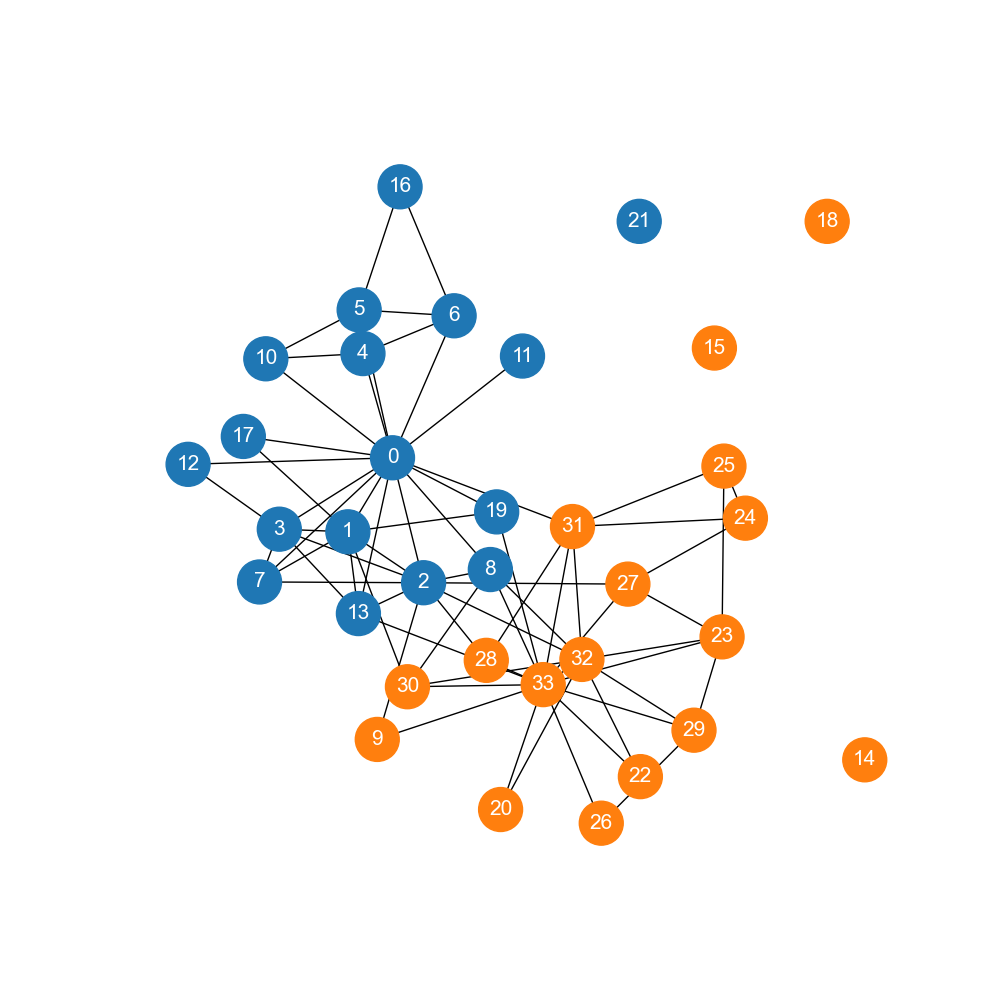
\includegraphics[width=.25\textwidth]{/files/src/.media/grafo_corte_24_2.0.png}}\hfill
    \\[\smallskipamount]
    \subfloat[av $\approx$ 2.00]{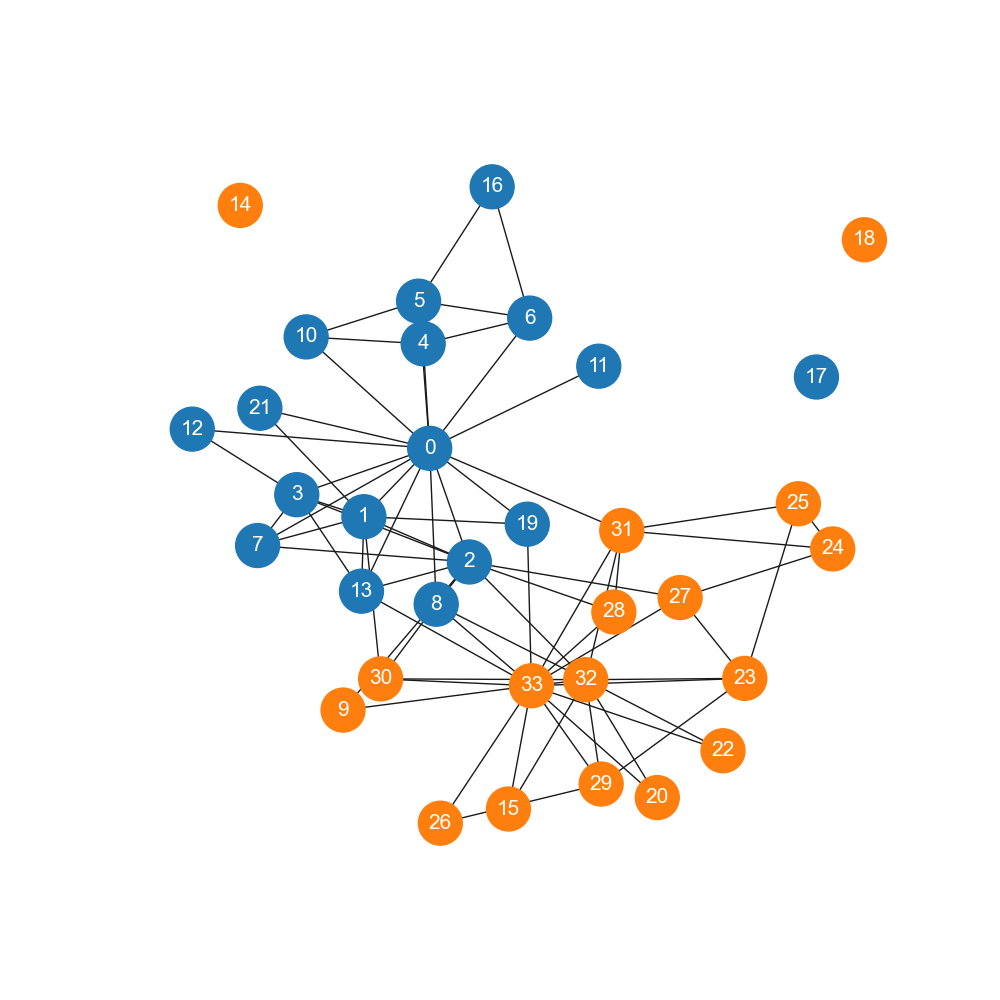
\includegraphics[width=.25\textwidth]{/files/src/.media/grafo_corte_23_2.0.png}}\hfill
    \subfloat[av $\approx$ 2.00]{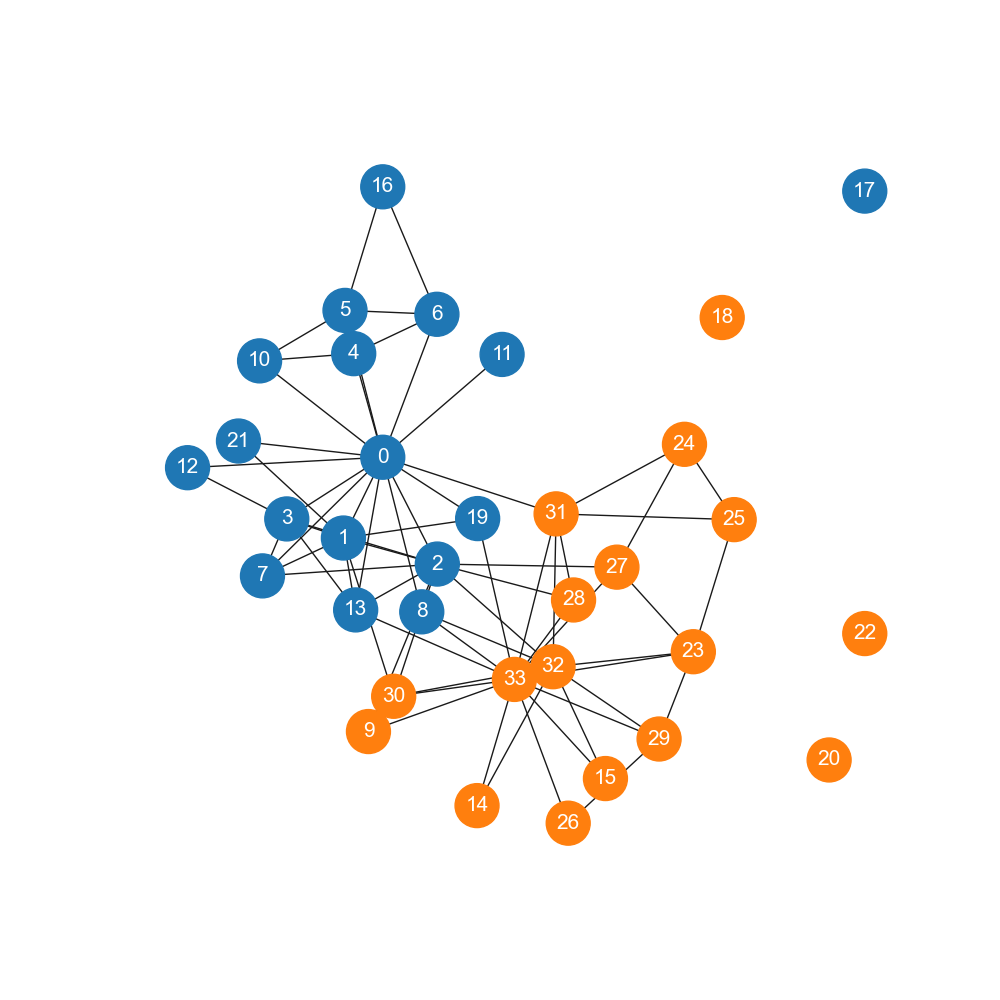
\includegraphics[width=.25\textwidth]{/files/src/.media/grafo_corte_22_2.0.png}}\hfill
    \subfloat[av $\approx$ 2.00]{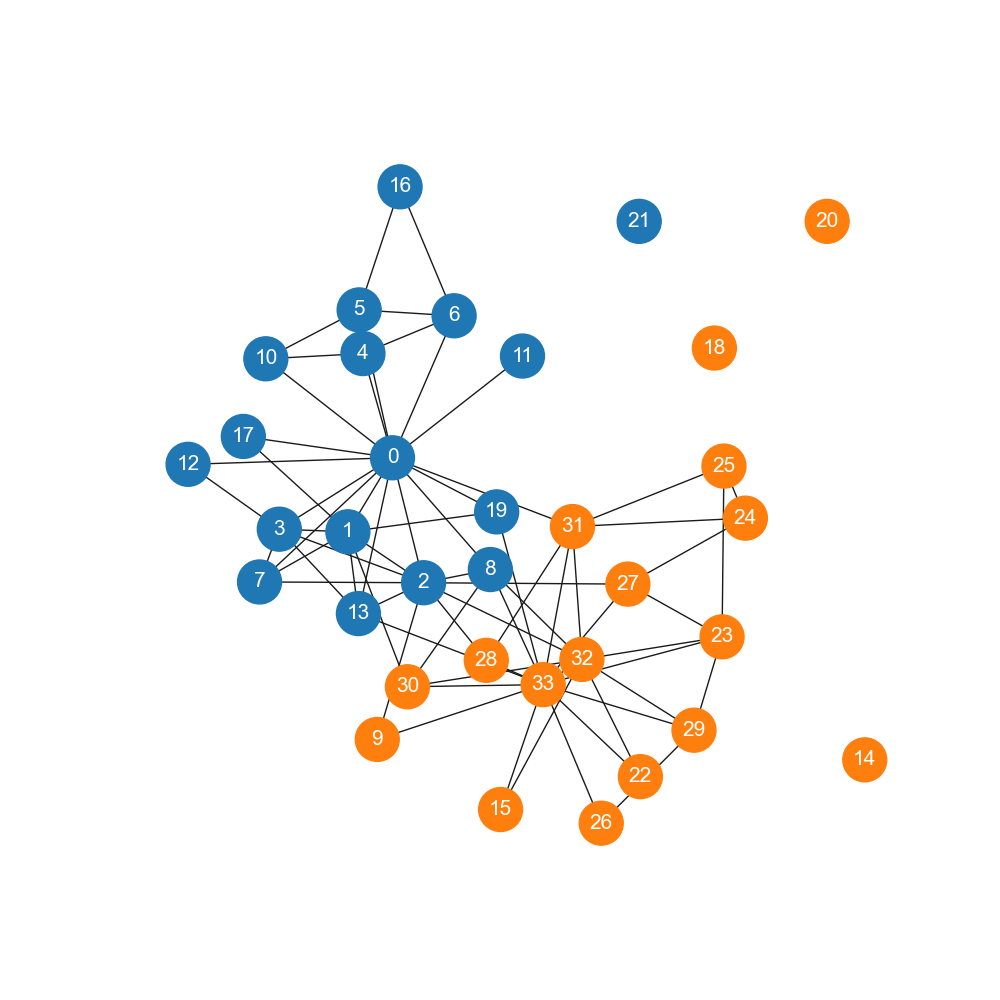
\includegraphics[width=.25\textwidth]{/files/src/.media/grafo_corte_21_2.0.png}}\hfill
    \subfloat[av $\approx$ 2.00]{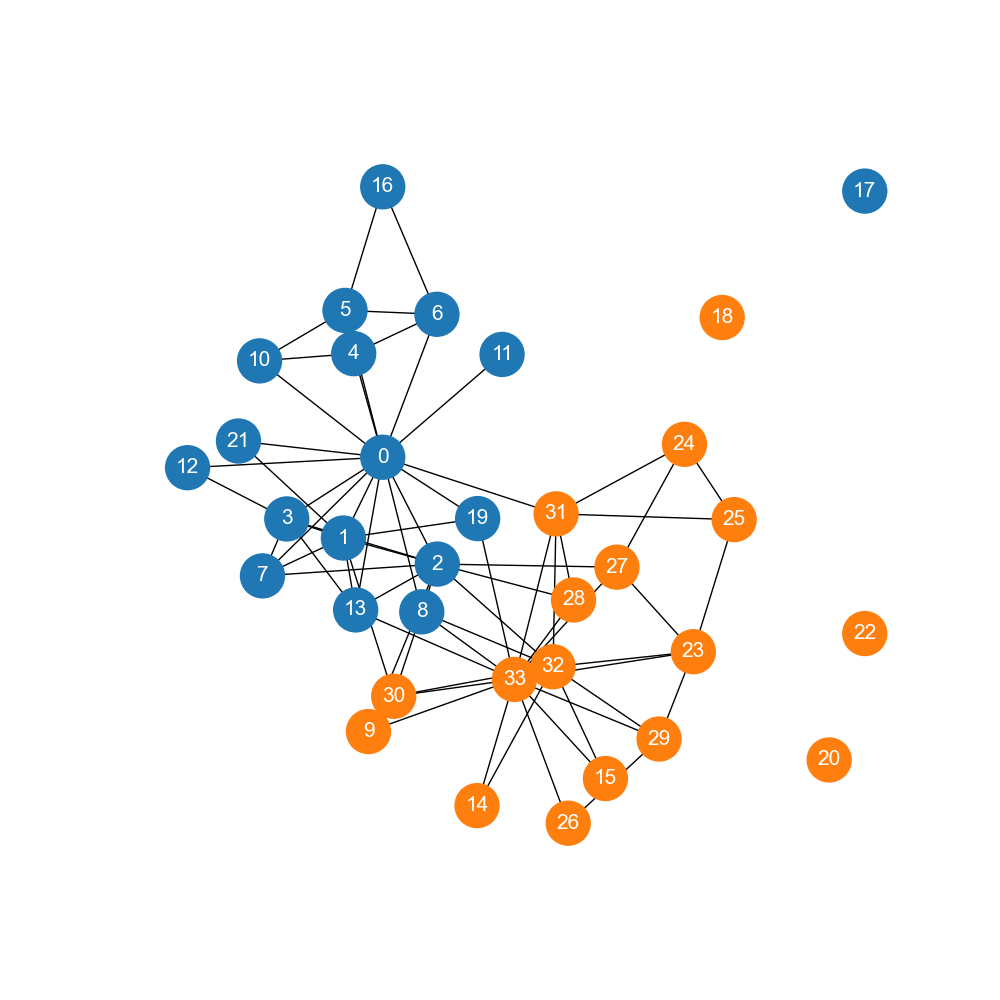
\includegraphics[width=.25\textwidth]{/files/src/.media/grafo_corte_20_2.0.png}}\hfill
    \\[\smallskipamount]
    \subfloat[av $\approx$ 2.49]{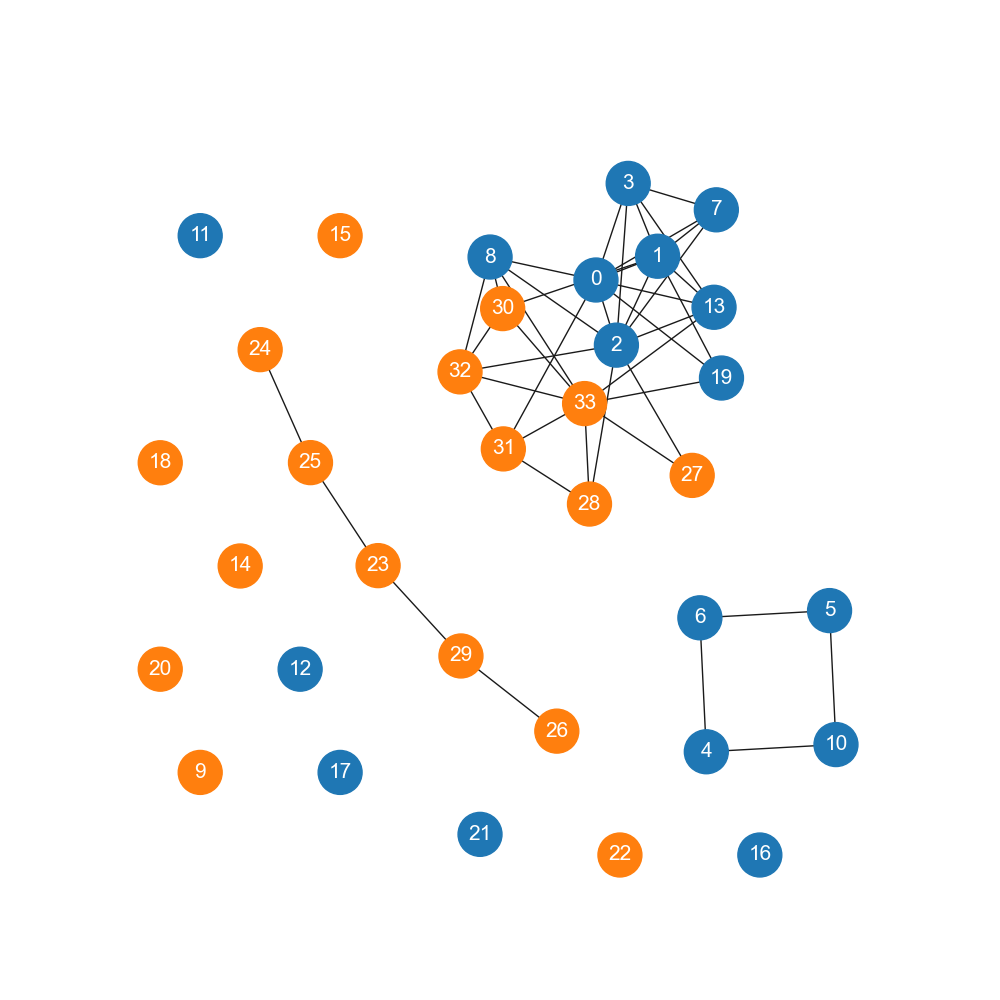
\includegraphics[width=.25\textwidth]{/files/src/.media/grafo_corte_19_2.49.png}}\hfill
    \subfloat[av $\approx$ 2.75]{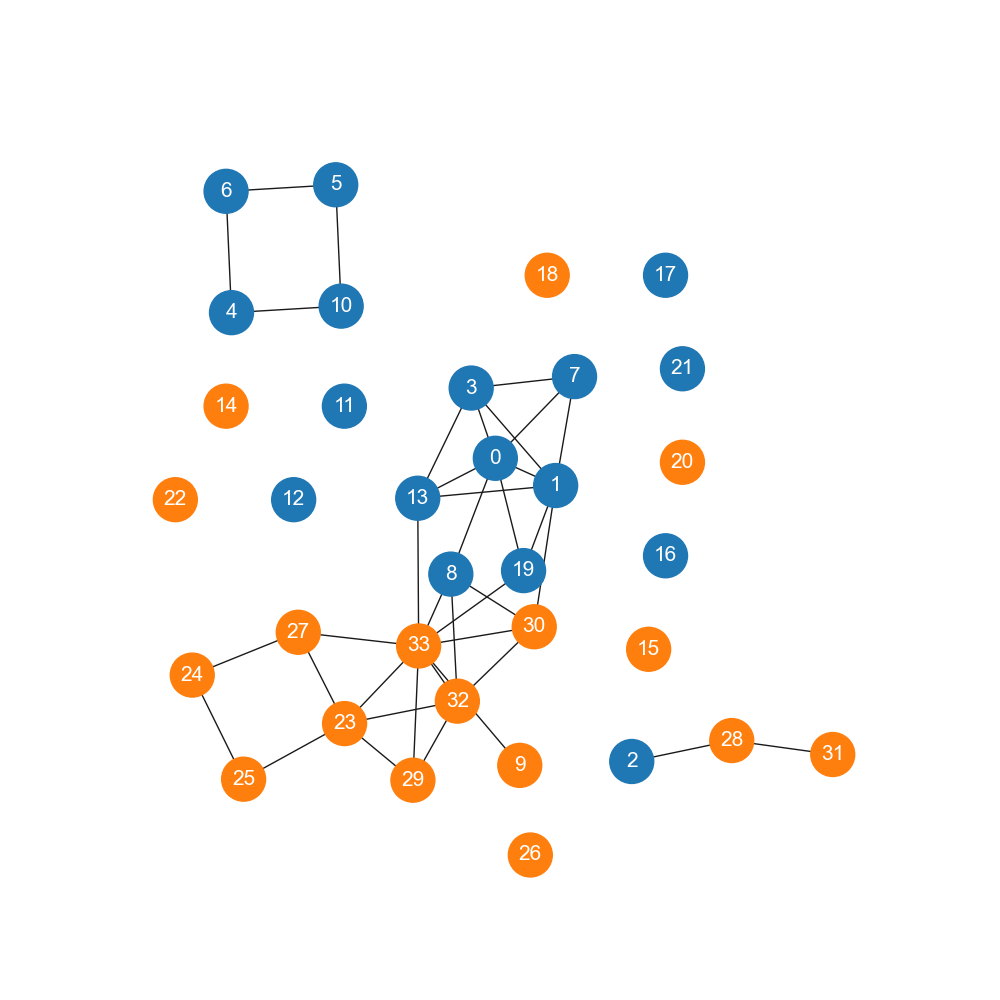
\includegraphics[width=.25\textwidth]{/files/src/.media/grafo_corte_18_2.75.png}}\hfill
    \subfloat[av $\approx$ 3.01]{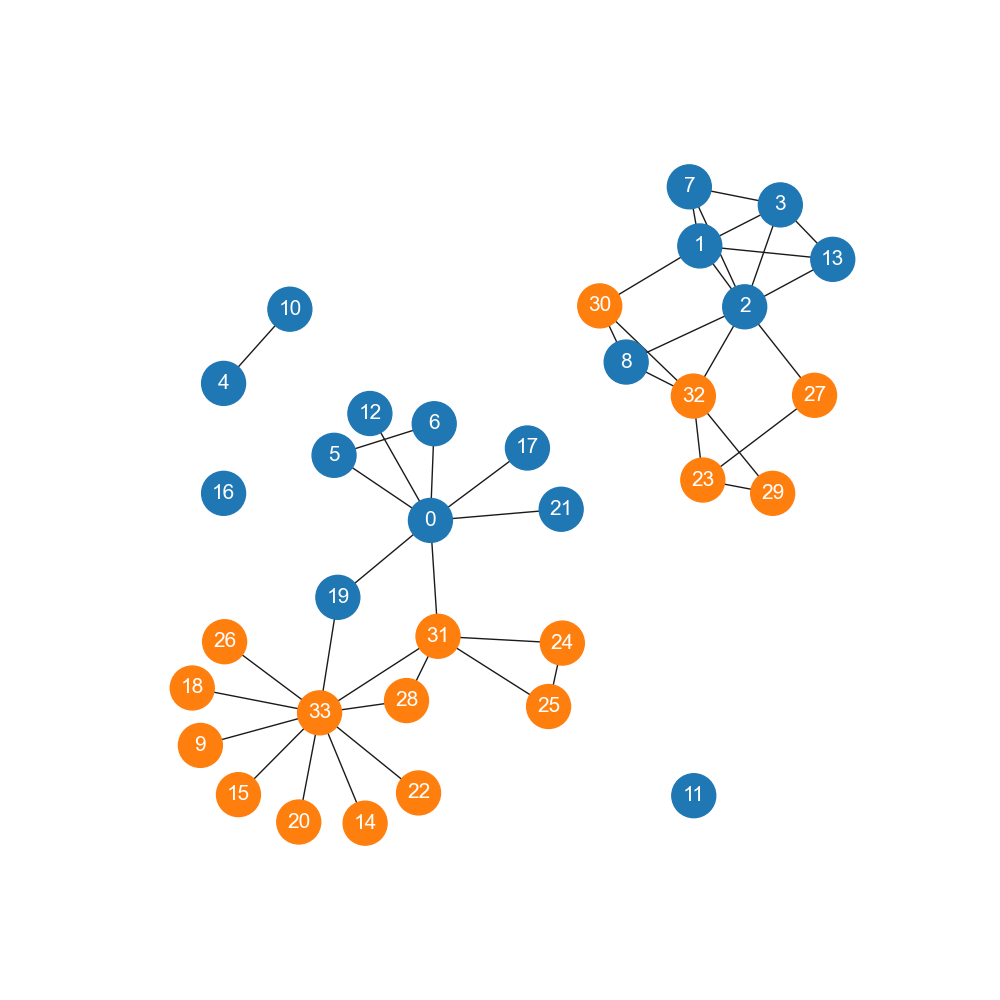
\includegraphics[width=.25\textwidth]{/files/src/.media/grafo_corte_17_3.01.png}}\hfill
    \subfloat[av $\approx$ 3.24]{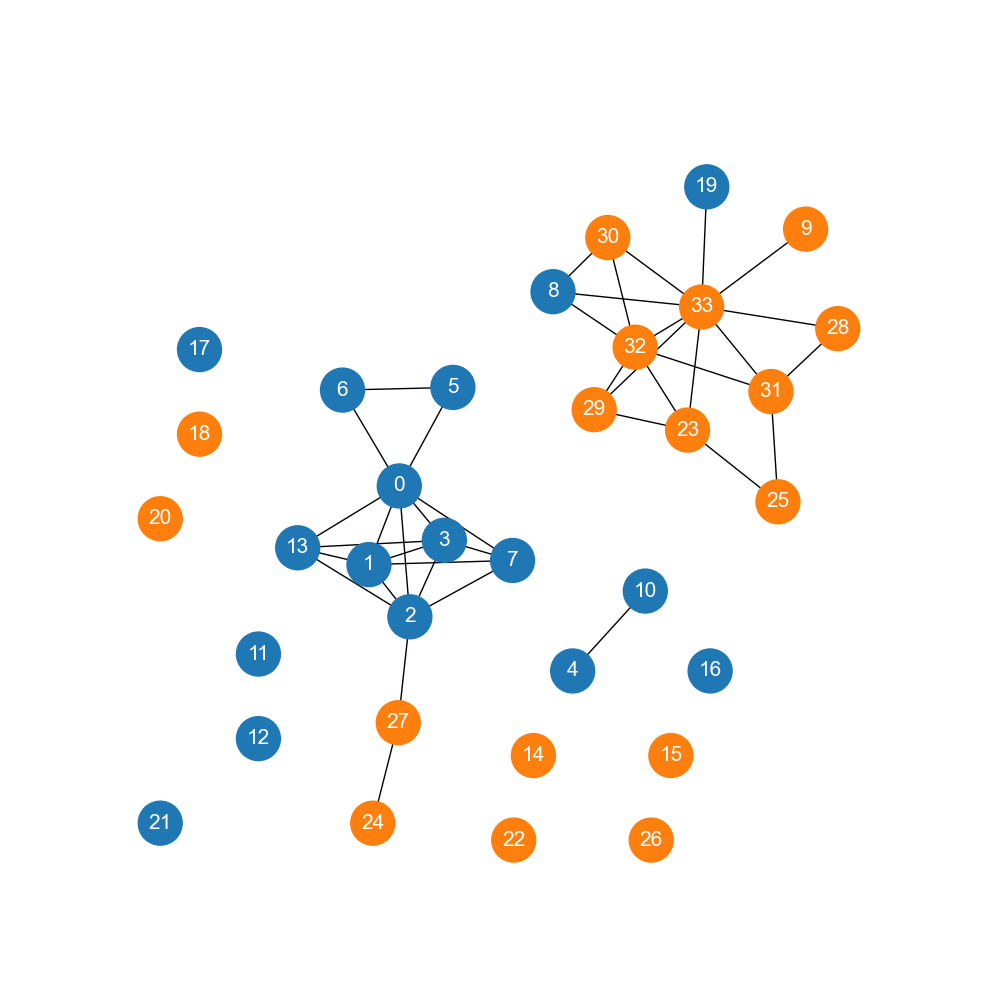
\includegraphics[width=.25\textwidth]{/files/src/.media/grafo_corte_16_3.24.png}}\hfill
\end{figure}

\begin{figure}[!htbp]
    \ContinuedFloat
    \centering
    \subfloat[av $\approx$ 3.38]{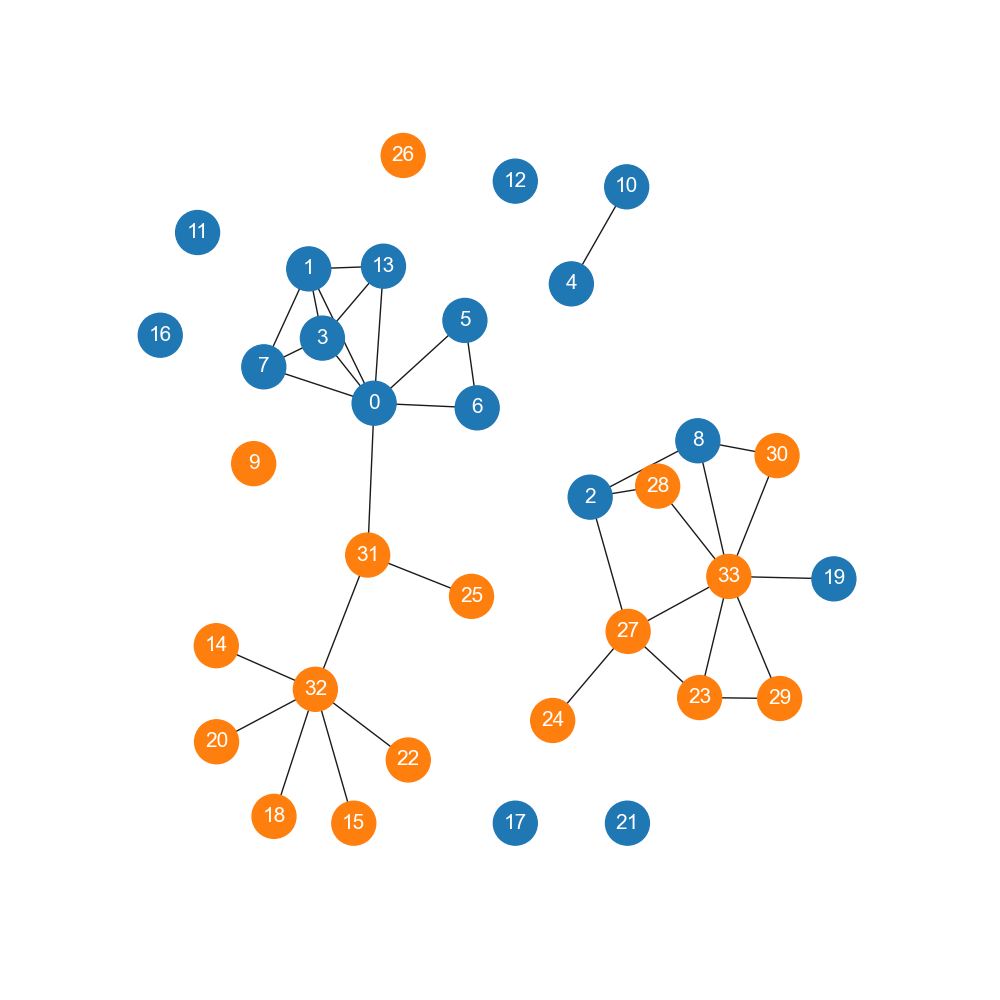
\includegraphics[width=.25\textwidth]{/files/src/.media/grafo_corte_15_3.38.png}}\hfill
    \subfloat[av $\approx$ 3.38]{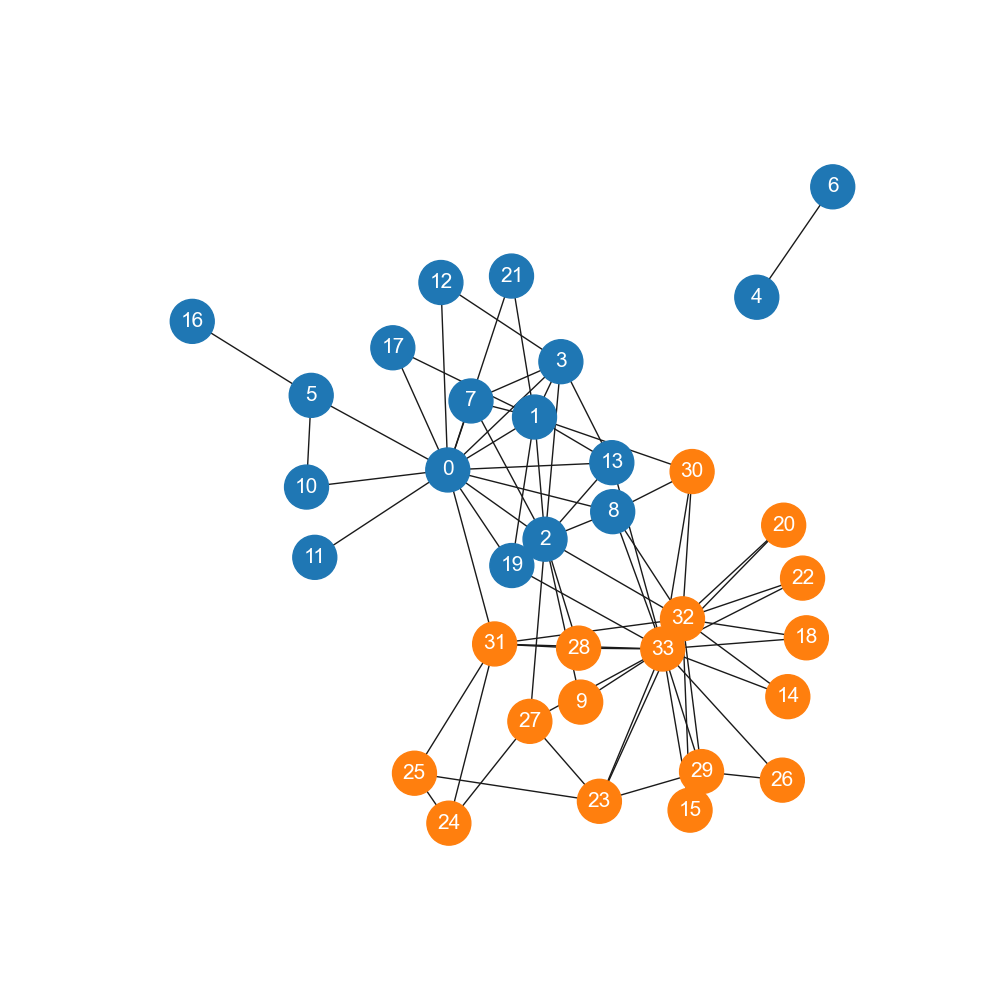
\includegraphics[width=.25\textwidth]{/files/src/.media/grafo_corte_14_3.38.png}}\hfill
    \subfloat[av $\approx$ 3.47]{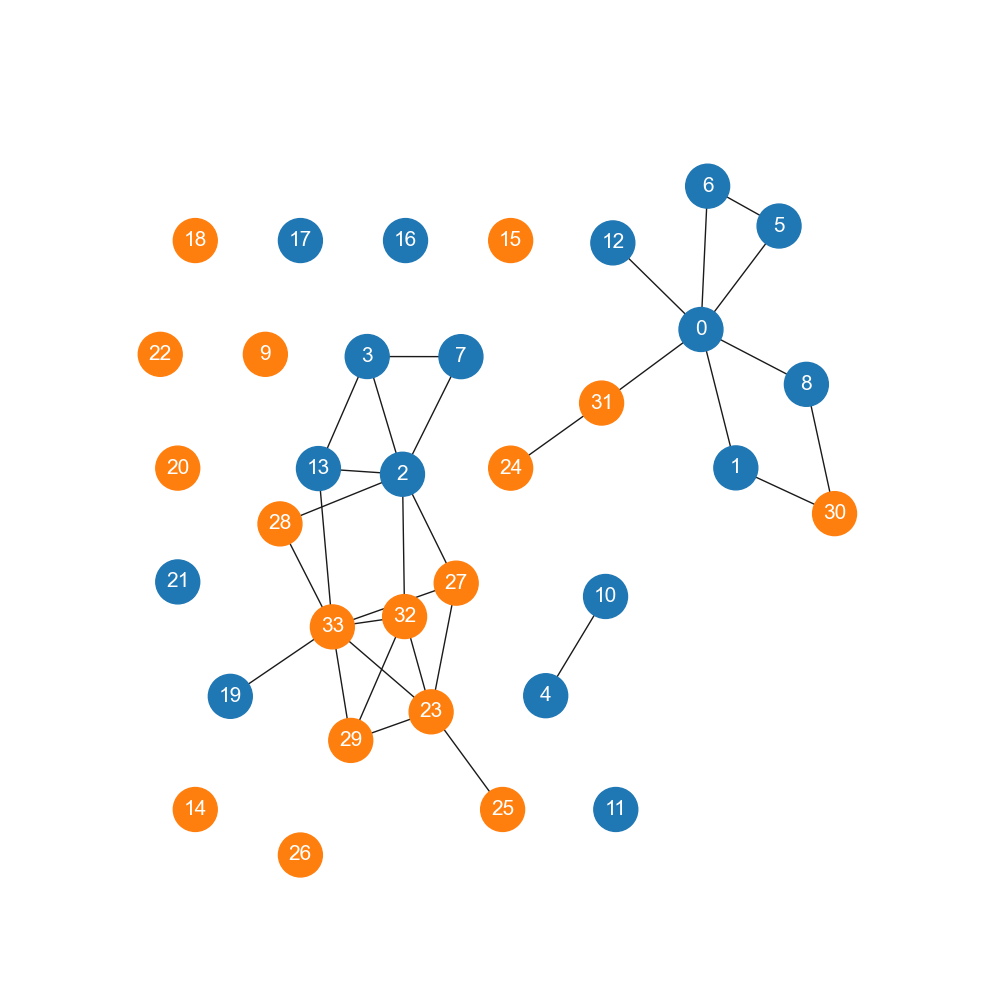
\includegraphics[width=.25\textwidth]{/files/src/.media/grafo_corte_13_3.47.png}}\hfill
    \subfloat[av $\approx$ 4.28]{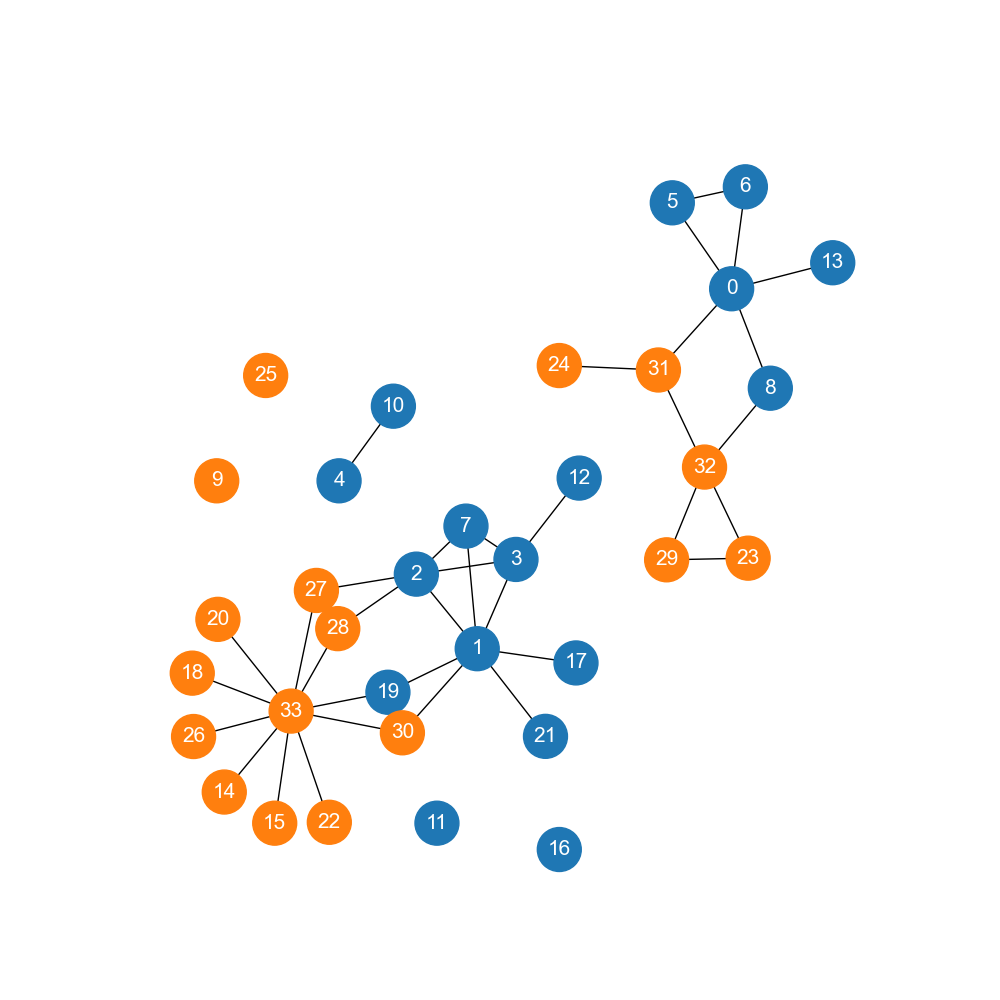
\includegraphics[width=.25\textwidth]{/files/src/.media/grafo_corte_12_4.28.png}}\hfill
    \\[\smallskipamount]
    \subfloat[av $\approx$ 4.48]{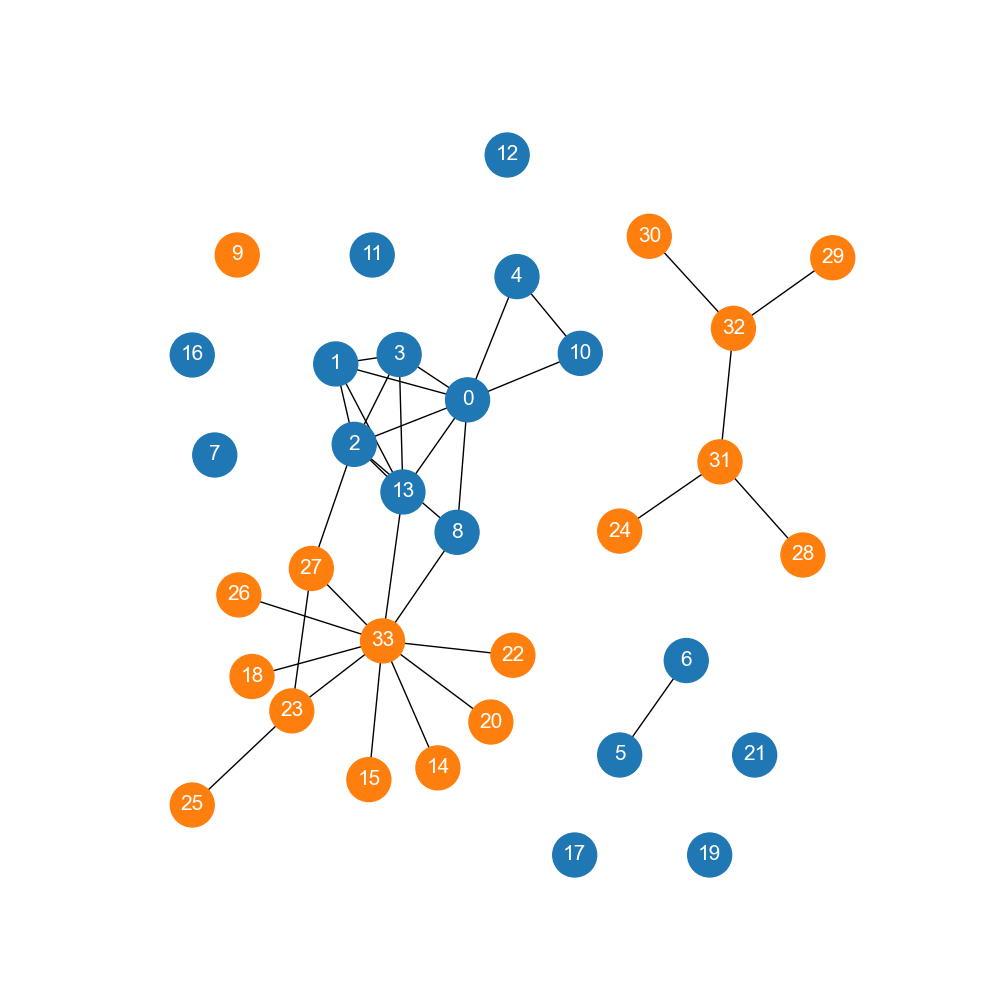
\includegraphics[width=.25\textwidth]{/files/src/.media/grafo_corte_11_4.48.png}}\hfill
    \subfloat[av $\approx$ 4.58]{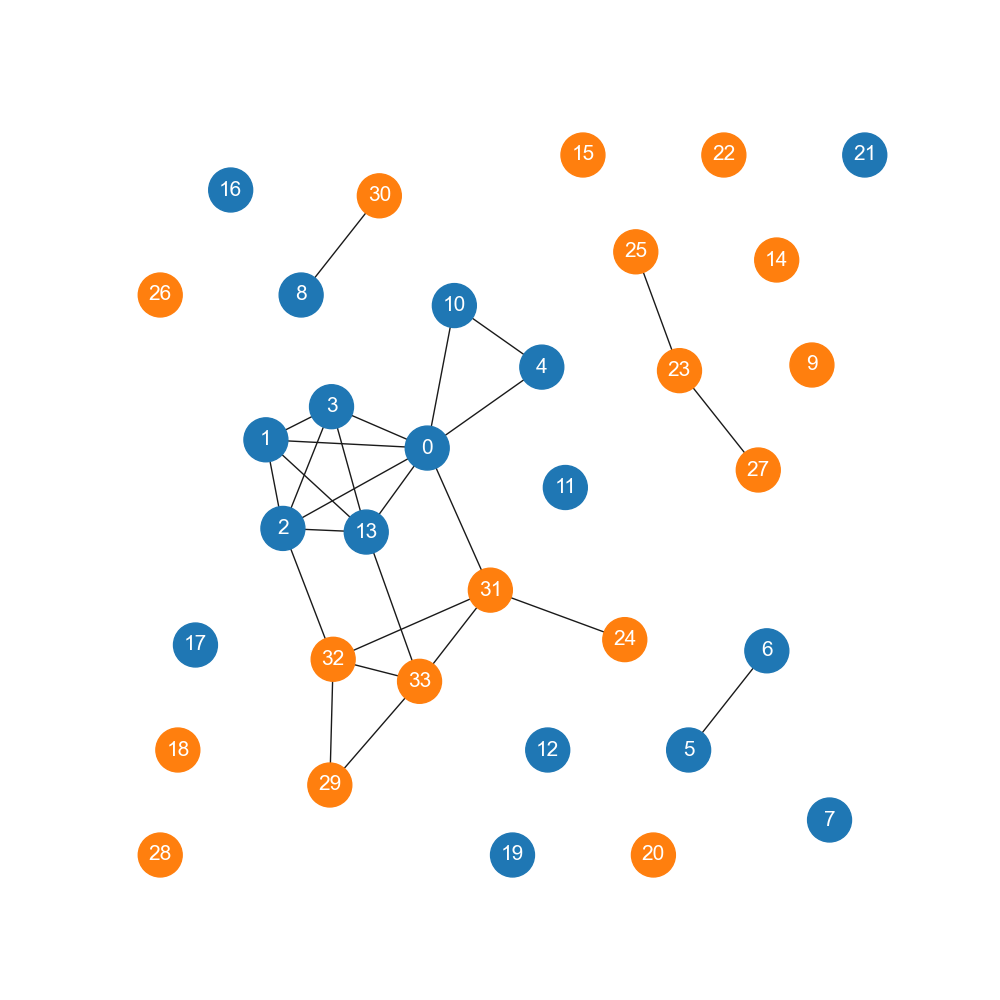
\includegraphics[width=.25\textwidth]{/files/src/.media/grafo_corte_10_4.58.png}}\hfill
    \subfloat[av $\approx$ 5.38]{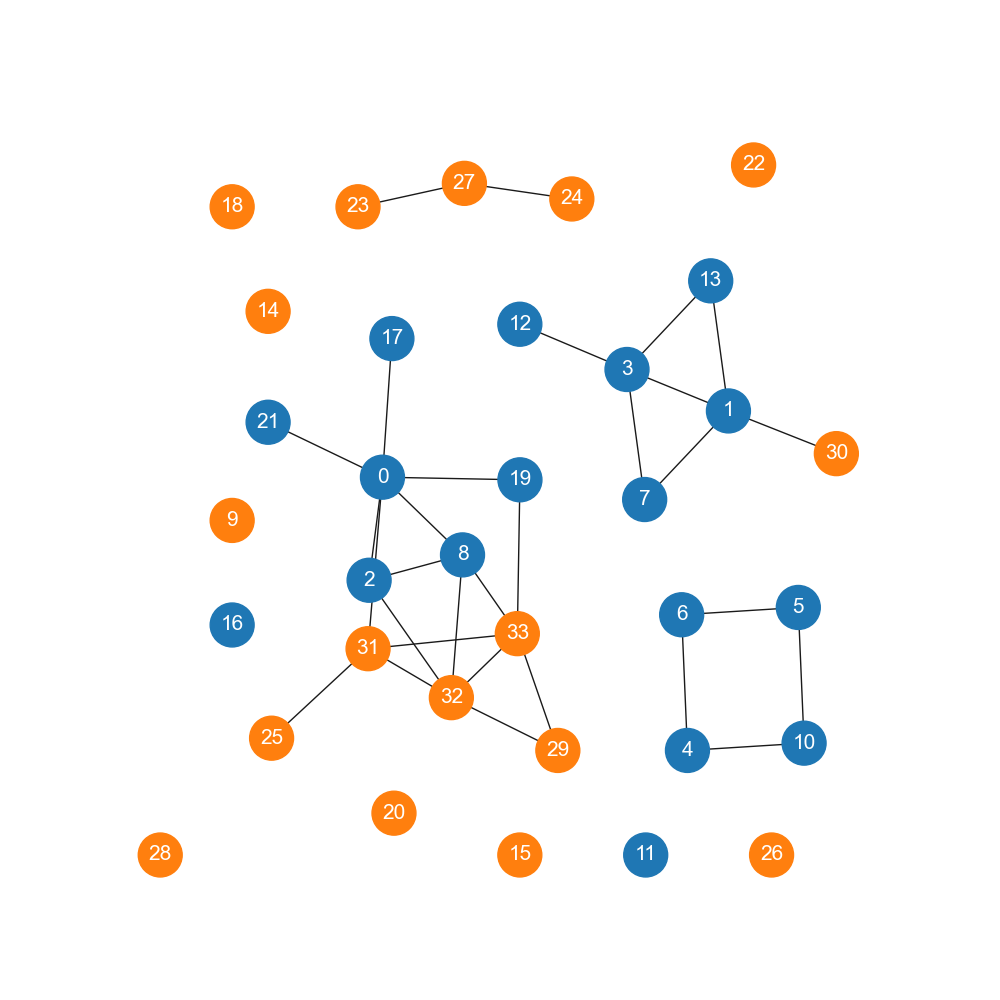
\includegraphics[width=.25\textwidth]{/files/src/.media/grafo_corte_9_5.38.png}}\hfill
    \subfloat[av $\approx$ 5.62]{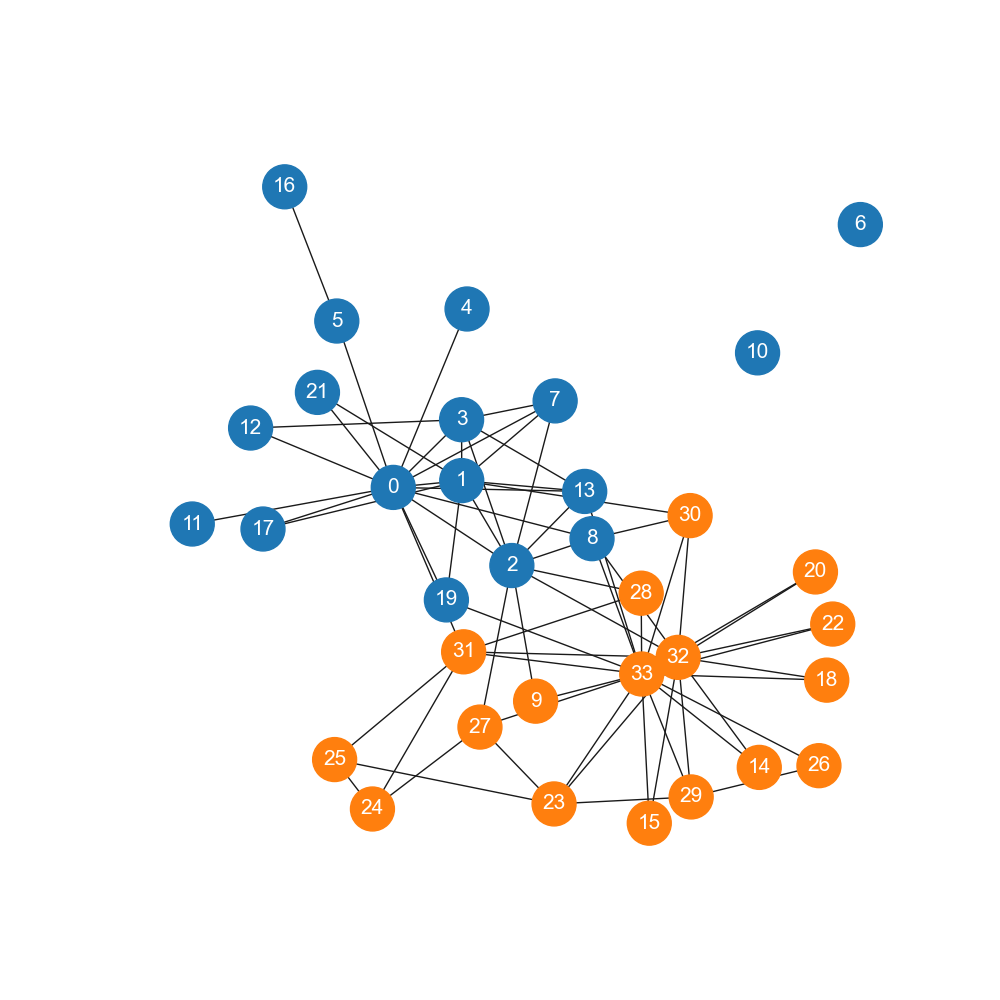
\includegraphics[width=.25\textwidth]{/files/src/.media/grafo_corte_8_5.62.png}}\hfill
    \\[\smallskipamount]
    \subfloat[av $\approx$ 6.33]{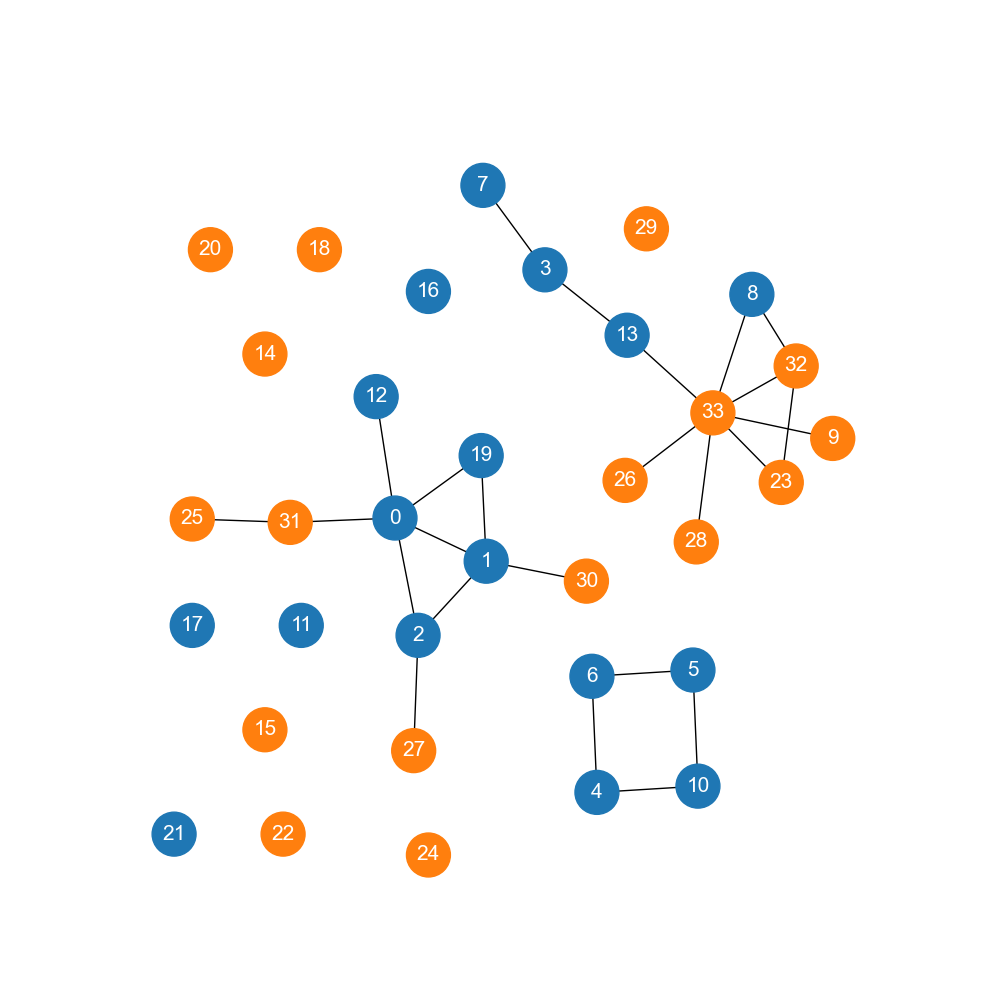
\includegraphics[width=.25\textwidth]{/files/src/.media/grafo_corte_7_6.33.png}}\hfill
    \subfloat[av $\approx$ 6.52]{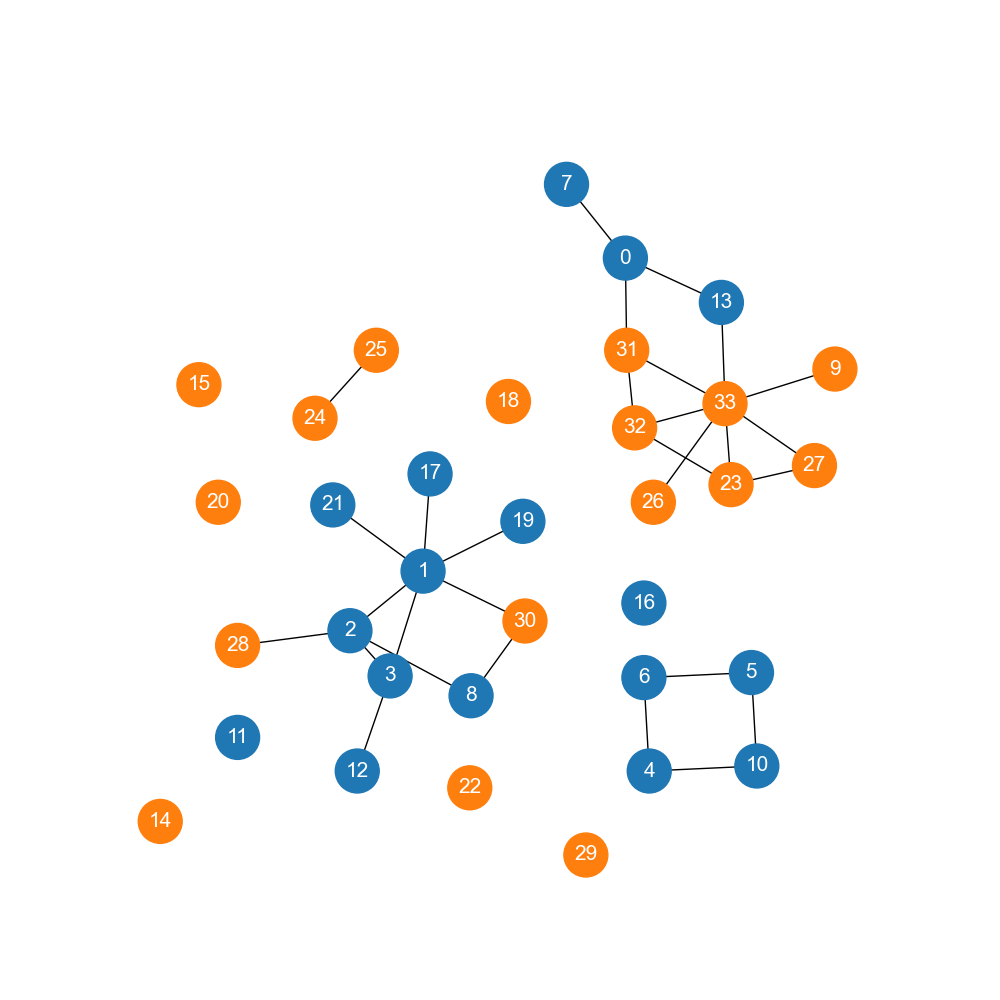
\includegraphics[width=.25\textwidth]{/files/src/.media/grafo_corte_6_6.52.png}}\hfill
    \subfloat[av $\approx$ 7.0]{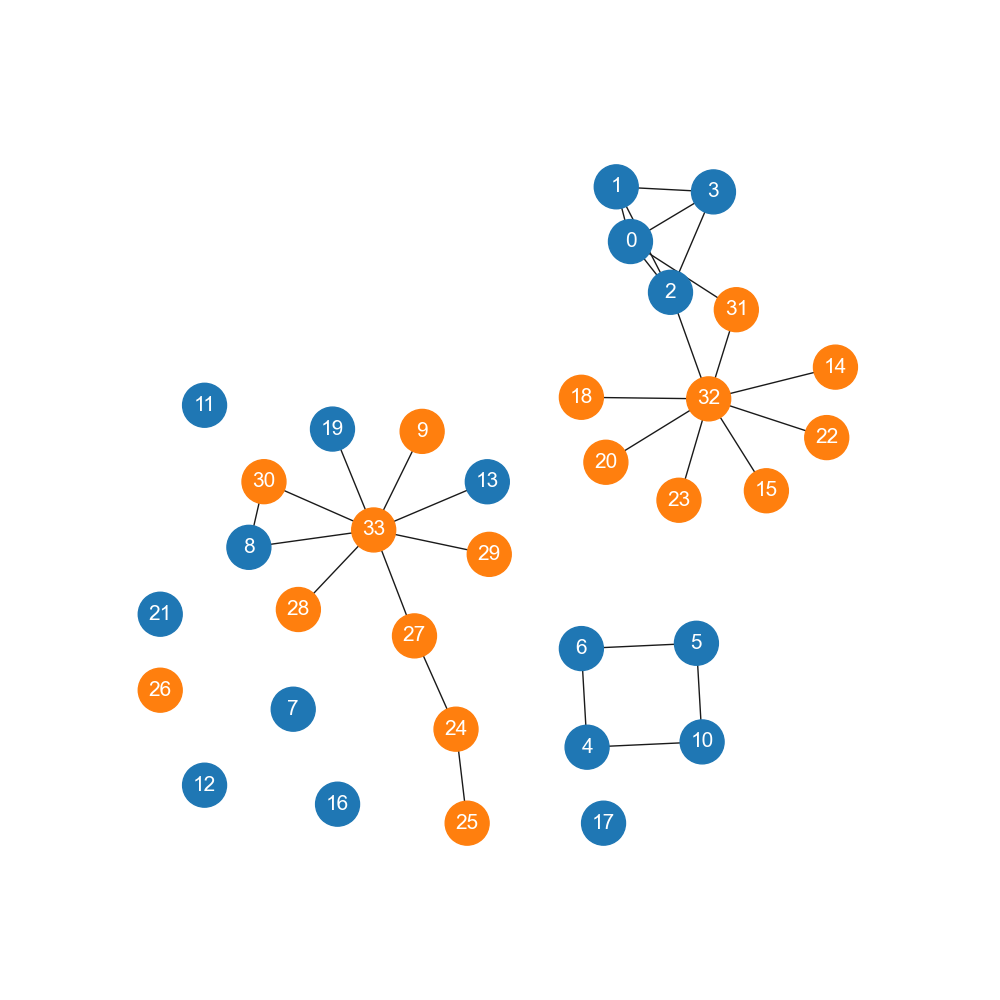
\includegraphics[width=.25\textwidth]{/files/src/.media/grafo_corte_5_7.0.png}}\hfill
    \subfloat[av $\approx$ 9.78]{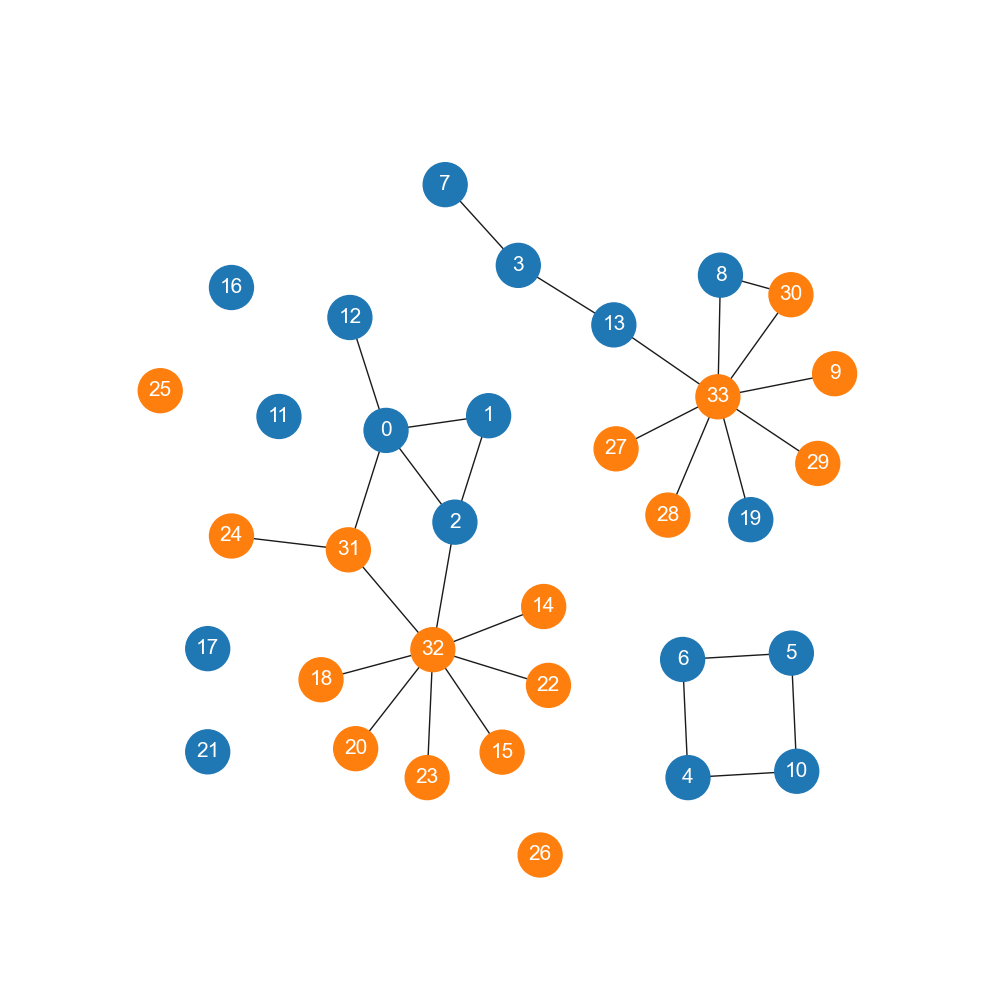
\includegraphics[width=.25\textwidth]{/files/src/.media/grafo_corte_4_9.78.png}}\hfill
    \\[\smallskipamount]
    \subfloat[av $\approx$ 10.92]{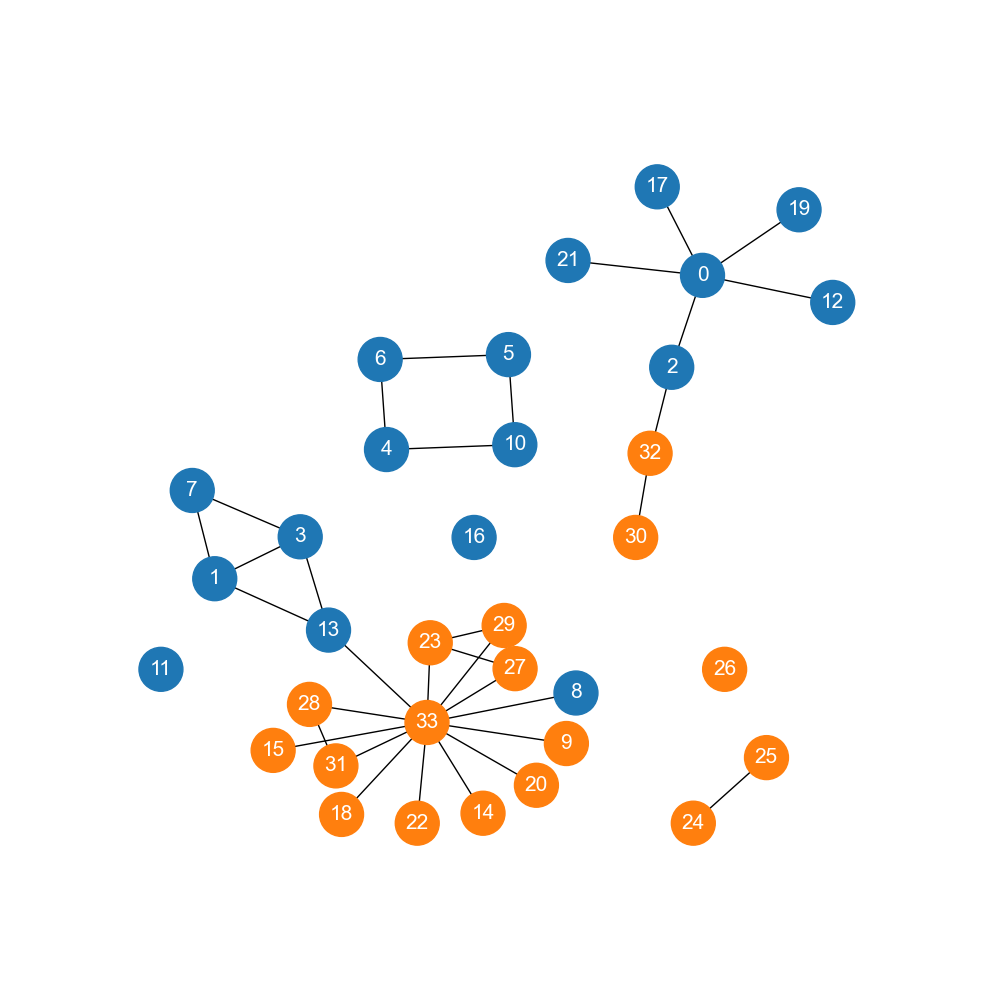
\includegraphics[width=.25\textwidth]{/files/src/.media/grafo_corte_3_10.92.png}}\hfill
    \subfloat[av $\approx$ 13.31]{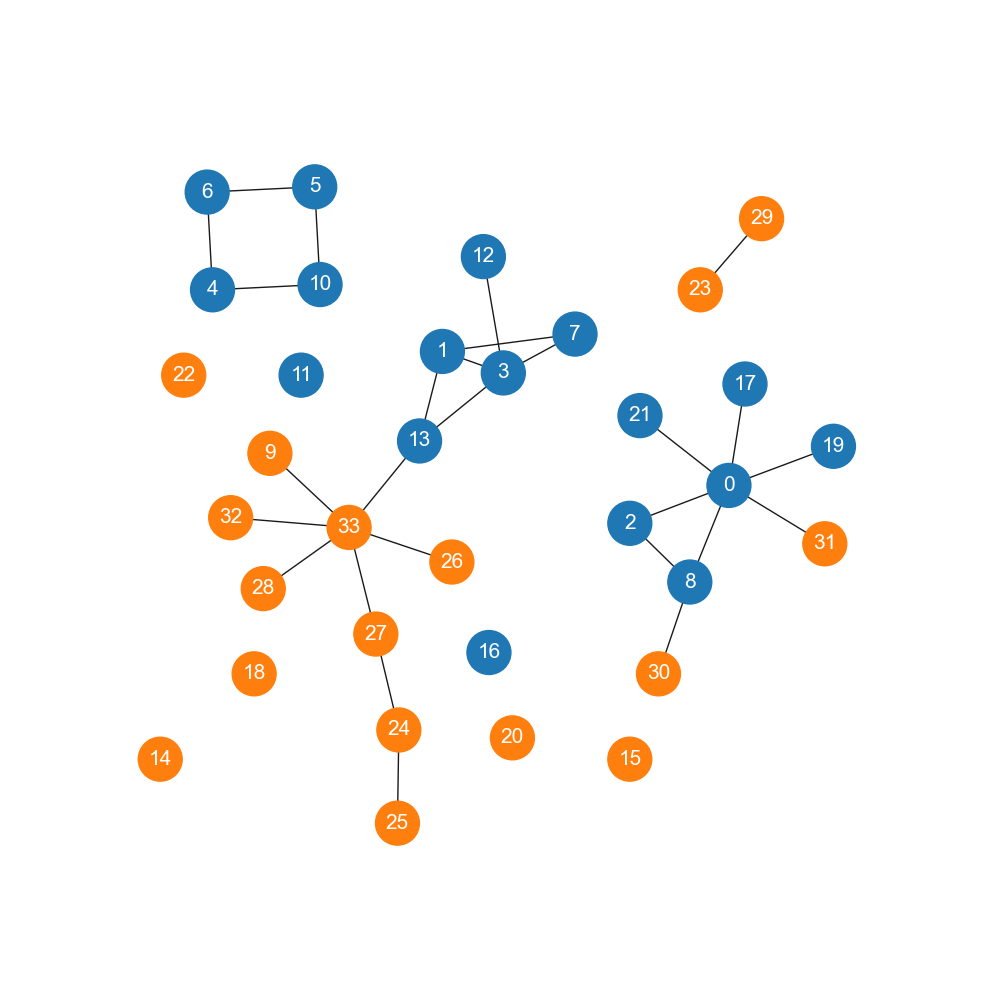
\includegraphics[width=.25\textwidth]{/files/src/.media/grafo_corte_2_13.31.png}}\hfill
    \subfloat[av $\approx$ 17.06]{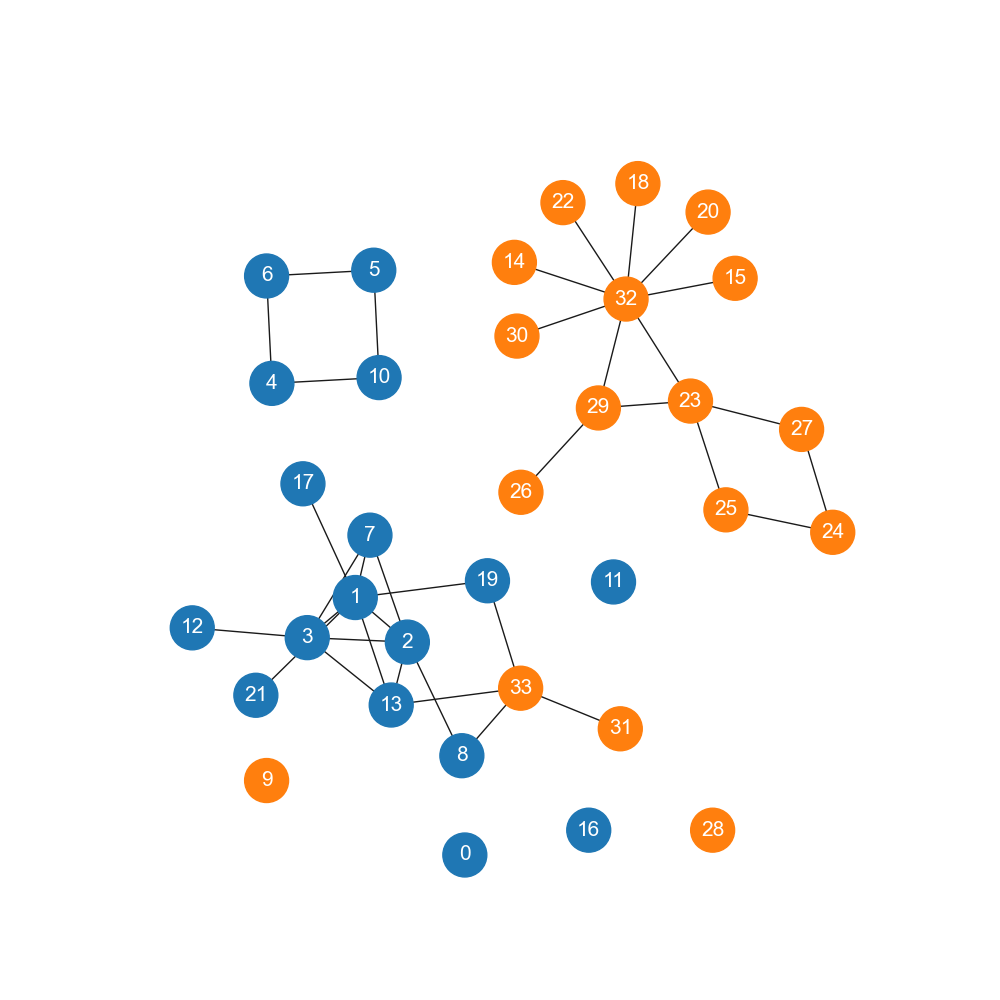
\includegraphics[width=.25\textwidth]{/files/src/.media/grafo_corte_1_17.06.png}}\hfill
    \subfloat[av $\approx$ 18.14]{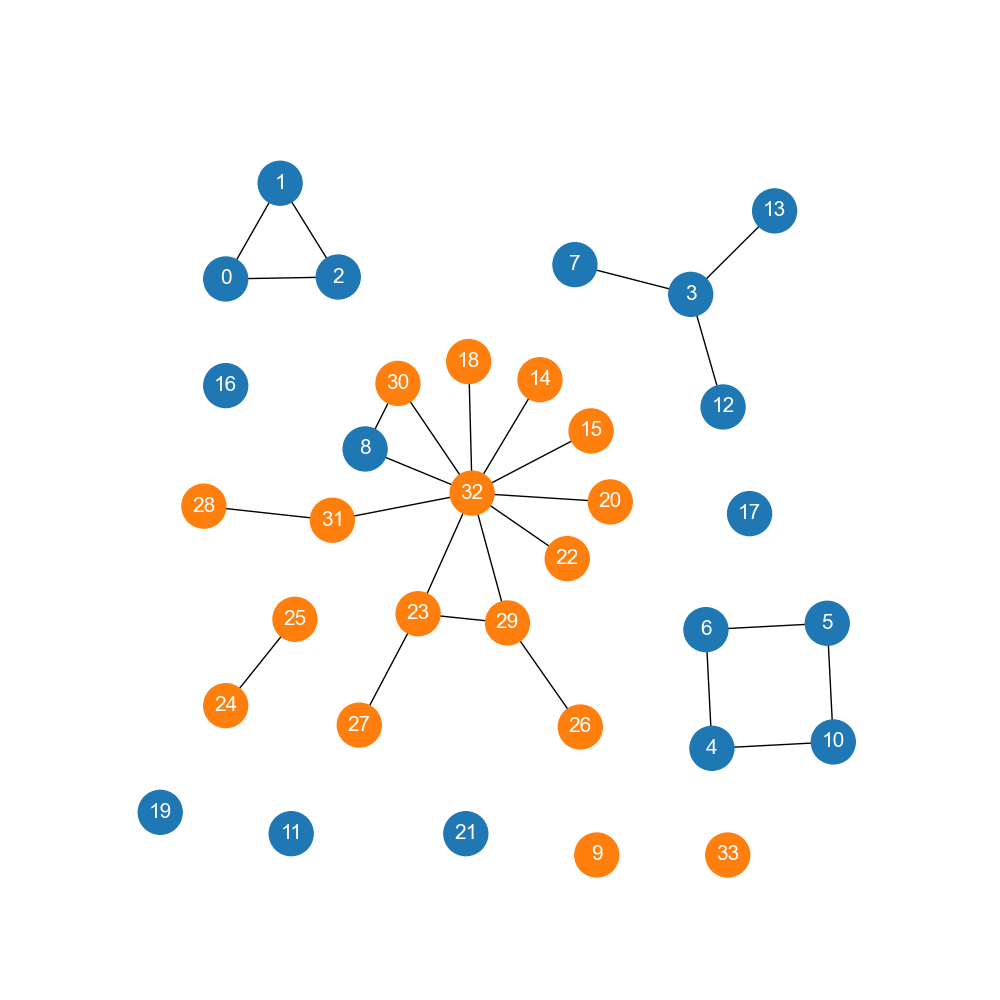
\includegraphics[width=.25\textwidth]{/files/src/.media/grafo_corte_0_18.14.png}}\hfill
    \\[\smallskipamount]
    \caption{Todos los cortes posibles ---salvo el de Fiedler y el nulo---, correspondientes a los autovectores asociados a la matriz laplaciana de la red del \textit{Club de Karate}. Cada uno se designa por medio de su autovalor.} \label{grafos_av}
\end{figure}
